\documentclass{article}
\usepackage{icml2026}
% Recommended, but optional, packages for figures and better typesetting:
\usepackage{microtype}
\usepackage{graphicx}
\usepackage{subcaption}
\usepackage{booktabs} % for professional tables
\usepackage[table]{xcolor} % for row colors in tables
\usepackage{enumitem}
% \usepackage{tcolorbox}
\usepackage{listings}
\usepackage{wrapfig}
\usepackage[most]{tcolorbox}
\tcbuselibrary{listings, breakable, skins}
\usepackage[pdfencoding=auto, psdextra, pagebackref=true]{hyperref}
\hypersetup{
    colorlinks,
    linkcolor={blue!50!black},
    citecolor={blue!50!black},
    urlcolor={blue!80!black}
}
% If you haven't defined these colors yet:
\definecolor{codebackground}{HTML}{F7F8FA}
\definecolor{codeborder}{HTML}{D9DDE3}

\tcbuselibrary{listings,skins,breakable}
% Define a style for code boxes
\definecolor{codebackground}{RGB}{248,248,248}
\definecolor{codeborder}{RGB}{200,200,200}


\tcbset{
  datasetbox/.style={
    enhanced,
    breakable,
    colback=codebackground,
    colframe=codeborder,
    boxrule=0.6pt,
    arc=2mm,
    left=2mm, right=2mm, top=1.2mm, bottom=1.2mm,
    fonttitle=\sffamily\small\bfseries,
    coltitle=black,
    attach boxed title to top left={xshift=1.5mm, yshift=-1.5mm},
    boxed title style={
      colback=codebackground,
      colframe=codeborder,
      boxrule=0.6pt,
      arc=1.5mm,
      left=1mm, right=1mm, top=0.6mm, bottom=0.6mm
    },
    before skip=4pt,
    after skip=6pt
  },
  jsonlisting/.style={
    listing only,
    listing engine=listings,
    listing options={%
      basicstyle=\ttfamily\small,
      breaklines=true,
      breakatwhitespace=false,
      columns=fullflexible,
      keepspaces=true,
      showstringspaces=false
    }
  }
}

\usepackage{amsmath}
\usepackage{amssymb}
\usepackage{mathtools}
\usepackage{amsthm}
\usepackage{multicol}
\usepackage{multirow}
\usepackage{xurl}


\theoremstyle{plain}
\newtheorem{theorem}{Theorem}[section]
\newtheorem{proposition}[theorem]{Proposition}
\newtheorem{lemma}[theorem]{Lemma}
\newtheorem{corollary}[theorem]{Corollary}
\theoremstyle{definition}
\newtheorem{definition}[theorem]{Definition}
\newtheorem{assumption}[theorem]{Assumption}
\theoremstyle{remark}
\newtheorem{remark}[theorem]{Remark}
\usepackage{xcolor}
\usepackage[table]{xcolor}
\definecolor{darkgreen}{rgb}{0.0,0.5,0.0}
\definecolor{lightblue}{RGB}{220,230,245}

\usepackage[textsize=tiny]{todonotes}

\icmltitlerunning{Draft-Conditioned Constrained Decoding for Structured Generation in LLMs}

\begin{document}

\twocolumn[
  \icmltitle{Draft-Conditioned Constrained Decoding for Structured Generation in LLMs}

  \icmlsetsymbol{equal}{*}

  \begin{icmlauthorlist}\icmlauthor{Anonymous}{anon}\end{icmlauthorlist}
  \icmlaffiliation{anon}{Anonymous Institution}
  
  % 

  \icmlcorrespondingauthor{Anonymous}{anonymous@anonymous.invalid}
  \icmlkeywords{Machine Learning, ICML}

  \vskip 0.3in
]

\printAffiliationsAndNotice{}  

\begin{abstract}
Large language models (LLMs) are increasingly used to generate executable outputs, JSON objects, and API calls, where a single syntax error can make the output unusable. Constrained decoding enforces validity token-by-token via masking and renormalization, but it can distort generation when the model assigns low probability mass to valid continuations, pushing decoding toward locally valid yet semantically incorrect trajectories. We propose \emph{Draft-Conditioned Constrained Decoding (DCCD)}, a simple two-step, training-free inference procedure that decouples semantic planning from structural enforcement: an unconstrained draft is generated first, and constrained decoding is then applied, conditioned on this draft, to guarantee validity. We analyze DCCD through a KL-projection view, showing that draft conditioning increases feasible mass and reduces the cumulative “projection tax” induced by hard constraints, with an optional best-of-$K$ draft selection. Across structured reasoning benchmarks, DCCD improves strict structured accuracy by up to +24 percentage points over standard constrained decoding (e.g., 15.2\% to 39.0\% on GSM8K with a 1B model), and enables smaller model pairs to match or exceed much larger constrained baselines, yielding substantial gains in parameter efficiency. We release code to reproduce all experiments at
\url{https://github.com/avinashreddydev/dccd}.
\end{abstract}


\section{Introduction}
\label{sec:intro}

Large language models (LLMs) are increasingly deployed not just as chatbots but as components in {software pipelines} that must produce {machine-interpretable outputs}. This shift is central to tool-augmented LLM systems and agentic workflows (e.g., Toolformer~\citep{schick2023toolformer}, ReAct~\citep{yao2022react}, MRKL-style tool routers~\citep{karpas2022mrkl}). In these settings, {syntactic validity is non-negotiable}, because a single missing brace in JSON, or an invalid SQL keyword, can cause downstream execution to fail. As a result, \emph{structured generation}, which produces outputs that must satisfy hard constraints such as JSON schemas, grammars, or tool-call formats, has become a practical bottleneck for reliable LLM deployment~\citep{agentkit}.
%
\begin{figure}[t]
    \centering
    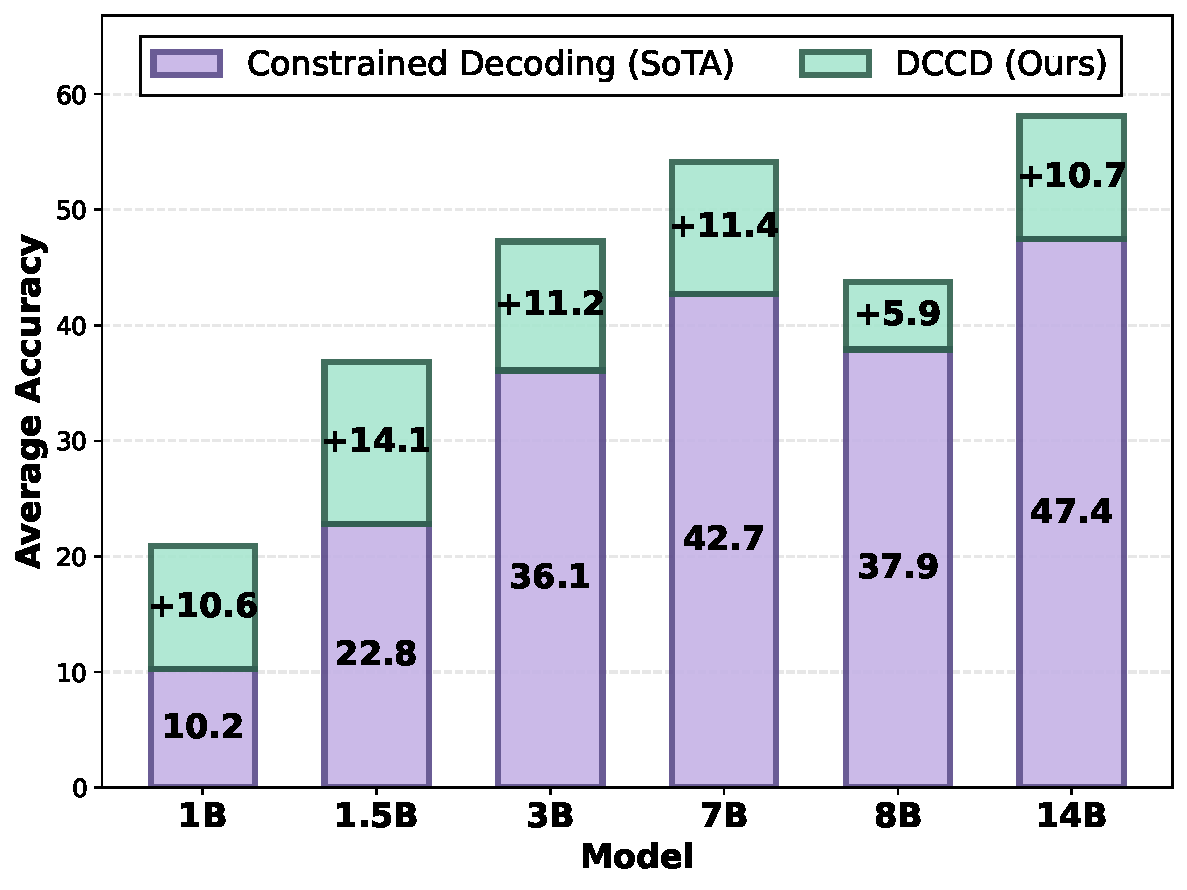
\includegraphics[width=\columnwidth]{figs/cd_dccd_accuracy_lift.pdf}
  \caption{Our proposed approach, Draft-Conditioned Constrained Decoding (DCCD), yields consistent accuracy improvements over standard constrained decoding (state of the art) across model scales (1B--14B). Purple bars denote baseline constrained decoding accuracy, while green segments show the absolute accuracy gain from DCCD. These gains reflect improved response correctness and structure adherence at all model sizes.}\vspace{-8mm}
    \label{fig:teaser}
\end{figure}

\textbf{Key existing approaches.} 
A first class of methods relies on {prompt-based format control} (schema instructions, few-shot demonstrations, and reminders {~\cite{elnashar2025prompt}.})
These can improve structural adherence, but they do not guarantee correctness and can still produce invalid outputs.
A second, widely used approach is \emph{constrained decoding} (CD), which enforces validity during generation by masking invalid tokens at every step. This includes lexically CD~\citep{hokamp-liu-2017-lexically, post-vilar-2018-fast}, finite-state CD~\citep{park2025flexible}, and systems that integrate grammar engines (e.g., PICARD for text-to-SQL~\citep{scholak-etal-2021-picard}) as well as more recent XGrammar~\citep{dong2025xgrammar} and Outlines~\citep{willard2023efficient}. Constrained decoding guarantees that every emitted token preserves global validity, so the final output response always satisfies the structural constraint.

\textbf{Challenge of constrained decoding.} 
Despite guaranteeing validity, constrained decoding often reduces semantic correctness on reasoning-intensive tasks~\citep{tam2024let, castillo2024, schall2025hidden}.
The root cause is that constrained decoding is not a passive formatting filter: it \emph{alters the model’s distribution at every token} by masking invalid tokens and renormalizing the remaining probability over the valid ones. When strict formats force low-entropy syntax decisions (e.g., braces, quotes, commas, or field names), the model may place only a little probability on the valid options at a prefix, so renormalization becomes a large perturbation. Repeating such perturbations across many steps induces a \emph{trajectory bias}: decoding is systematically pushed toward prefixes that are easier to keep valid, even when they correspond to an incorrect underlying solution.


\textbf{Our key insight.}
The severity of this distortion is not intrinsic to the constraint alone, it depends on the \emph{context} the model is conditioned on. If we can first supply a semantic plan that makes schema-consistent continuations likely, then the same hard constraints become far less distortive. This motivates a simple strategy: rather than forcing the model to \emph{reason inside} the constraint set, we first generate an unconstrained draft (capturing the semantic plan) and then apply constrained decoding \emph{conditioned on the draft} to guarantee validity. This “draft-then-constrain” approach reduces constraint-induced distortion while preserving exact structural guarantees.

\textbf{Our solution.}
Motivated by this view, we propose Draft-Conditioned Constrained Decoding (DCCD), a lightweight, training-free two-step inference procedure. In Step~1, a model generates an \emph{unconstrained draft} that captures the semantic plan or intermediate reasoning. In Step~2, we generate the final structured output using constrained decoding \emph{conditioned on the draft}.
Conditioning shifts probability mass toward schema-consistent continuations, so the subsequent constraint enforcement step is
substantially less distortive. Because Step~2 primarily performs \emph{structured realization} rather than open-ended reasoning, it can often be carried out by
the same model or a smaller projector model, improving parameter efficiency.
We summarize our contributions as follows.

$\bullet$ \textbf{Highlighting why constrained decoding fails.}
    We present a KL-projection perspective of constrained decoding and show that constraint-induced distortion is governed by the probability mass assigned to valid continuations (feasible mass), yielding a cumulative ``projection tax'' and trajectory-dependent bias under hard constraints.

  
  $\bullet$ \textbf{Draft-Conditioned Constrained Decoding (DCCD).}
    We introduce a training-free two-step inference algorithm that generates an unconstrained draft (semantic plan) and then performs constrained decoding conditioned on the draft, increasing feasible mass \emph{before} enforcing hard constraints while retaining exact validity guarantees. We also show the test-time scaling effectiveness of the DCCD approach. 

        $\bullet$ \textbf{Empirical results.} Across multiple structural constraint types (JSON schemas, expression grammars, and prover-checked logical forms) and reasoning benchmarks (GSM8K, MATH500, GSM-Symbolic, and FOLIO/P-FOLIO), DCCD consistently improves \emph{strict structured accuracy} (correct \emph{and} valid) and enables parameter-efficient two-model compositions that outperform larger single-model constrained baselines. For example, under a strict JSON constraint on GSM8K, DCCD improves a 1B model from 15.24\% to 39.0\% strict accuracy, and improves a 1.5B model from 49.36\% to 73.92\%.

\section{Related Works}
 The landscape of constrained decoding spans several algorithmic paradigms. Early work on lexically constrained decoding~\citep{hokamp-liu-2017-lexically, post-vilar-2018-fast} enforced specific word or phrase inclusion in neural machine translation. This evolved into grammar-based approaches that integrate incremental parsing or automaton engines to enforce context-free grammars~\citep{scholak-etal-2021-picard, park2025flexible}. Modern structured decoding systems~\citep{willard2023efficient, dong2025xgrammar,suresh2025dingo,ugare2024itergen,ugare2024syncode,openaistructuredoutputs2024} extend these ideas to JSON schemas, type systems, and domain-specific languages, achieving efficient token-level filtering through optimized finite-state machines and parser integration. These systems are widely deployed in production LLM APIs~\citep{openaistructuredoutputs2024, claudestructuredoutputs2024} and form the backbone of tool-calling infrastructure.

Recent works~\citep{tam2024let, castillo2024, schall2025hidden} have documented performance degradation by 10-30\% compared to unconstrained generation under hard structural constraints. Several approaches attempt to reduce this semantic distortion. Interleaved reasoning frameworks~\citep{banerjee2025crane} allow models to alternate between free-form reasoning and structured generation, deferring structure until reasoning is complete. However, when structure is required from the first token, as in tool calls or API arguments, these methods reduce to standard constrained decoding, inheriting the same quality-validity tradeoff. \textbf{Our work} argues that the quality--validity trade-off is largely an artifact of {how} constraints are enforced at inference time.
We show that one can preserve exact structural guarantees while matching (or approaching) unconstrained task accuracy, without relaxing the constraint set.


\section{Problem Formulation}
\label{sec:problem}
%
Let $x$ denote an input prompt and let $z_{1:T}$ denote an output token sequence of length $T$ over a vocabulary $\mathcal{V}$.
A pretrained autoregressive language model $\pi_{\theta}$ (base model) induces the sequence distribution
\begin{align}
\rho_\theta(z_{1:T}\mid x) \;=\; \prod_{t=1}^{T} \pi_{\theta}(z_t \mid h_t),
\qquad
h_t \triangleq (x, z_{<t}).
\end{align}
%
\textbf{Hard structural constraints.}
We consider {hard} (non-negotiable) constraints that define a set of {valid} outputs.
Formally, let $\mathcal{L}(x)\subseteq \mathcal{V}^\star$ denote the set of all sequences that satisfy the required structure for input $x$
(e.g., a JSON schema, a context-free grammar, a tool-call signature, or a proof/program syntax).
%
A standard way to represent such constraints is via the {valid-next-token set}.
For each state $h_t=(x,z_{<t})$, we define
\begin{align}
A(h_t) \;\triangleq\; \{a\in\mathcal{V}:\ & \exists \text{ a completion } z_{t+1:T} \text{ s.t. } \nonumber
\\
&\quad \quad \quad (z_{<t},a,z_{t+1:T})\in\mathcal{L}(x)\}.
\label{eq:valid_next_tokens}
\end{align}
Equivalently, one can define a prefix-dependent binary mask $m_t\in\{0,1\}^{|\mathcal{V}|}$ with
$m_t(a)=\mathbb{I}[a\in A(h_t)]$ for $a\in\mathcal{V}$.
This abstraction covers grammar-constrained decoding, JSON-schema constrained generation, and executable-output formats used in semantic parsing and tool calling
(e.g., lexically constrained decoding , finite-state constrained decoding ~\citep{willard2023efficient, dong2025xgrammar,suresh2025dingo,ugare2024itergen,ugare2024syncode,openaistructuredoutputs2024} , and incremental parsing constraints such as PICARD \citep{scholak-etal-2021-picard}. 

\textbf{Objective.}
The goal is to generate a response from the language model $\pi_{\theta}$ for a given $x$ that always satisfies the structure constraint while preserving task utility.
Let $U(x,z)$ denote a task-specific utility (e.g., exact-match accuracy, execution success, or prover verification).
We aim to produce a constrained distribution $q$ over sequences such that $q$ is supported on $\mathcal{L}(x)$ and attains high expected utility:
\begin{align}
\max_{q}\;\; \mathbb{E}_{z\sim q}\!\left[U(x,z)\right]
\quad\text{s.t.}\quad
q(z\notin\mathcal{L}(x))=0.
\label{eq:utility_goal}
\end{align}
Because $U(\cdot)$ is typically unavailable at inference time, most practical methods (e.g., constraint decoding) enforce constraints while attempting to stay close to the base model distribution.

%
\subsection{Existing Approach: Constrained Decoding}
\label{sec:mask_proj}
The standard constrained decoding approaches  \citep{hokamp-liu-2017-lexically, post-vilar-2018-fast, willard2023efficient, dong2025xgrammar} enforces constraints {during generation} by masking invalid tokens and renormalizing at each step
.
Concretely, it defines the constrained per-step distribution
%
\begin{align}
q(z_t \mid h_t)
\;=\;
\frac{\pi_{\theta}(z_t\mid h_t)\,\mathbb{I}[z_t\in A(h_t)]}{\alpha(h_t)},
\label{eq:mask_renorm}
\end{align}
%
where $\alpha(h_t)\triangleq \sum_{a\in A(h_t)} \pi_{\theta}(a\mid h_t),$  is the feasible mass at step $t$.  We call $\alpha(h_t)$ the feasible mass because it is the total probability that the model assigns to feasible (i.e., constraint-valid) next tokens for a given $h_t$. Then, we sample $z_t\sim q(\cdot\mid h_t)$ (or greedily takes $\arg\max$ under $q$), guaranteeing that the final output lies in $\mathcal{L}(x)$. 

The quantity $\alpha(h_t)$ is the {feasible mass} that the base model assigns to valid continuations at prefix $h_t$.
Masking and renormalization introduce a per-step reverse-KL distortion
%
\begin{align}
\mathrm{KL}\!\left(q(\cdot\mid h_t)\,\|\pi_\theta(\cdot\mid h_t)\right)
\;=\;
\log\frac{1}{\alpha(h_t)}.
\label{eq:kl_log_alpha}
\end{align}
%
Thus, whenever $\alpha(h_t)\ll 1$, constrained decoding substantially reshapes the distribution over the remaining valid tokens. Further, aggregating across time yields a sequence-level projection tax. Let $\rho_q(z_{1:T}\mid x)\triangleq \prod_{t=1}^T q(z_t\mid h_t)$ denote the constrained autoregressive factorization induced by \eqref{eq:mask_renorm}.
Then the total distortion relative to the base model admits the identity
\begin{align}
\text{KL}\!\left(\rho_q(\cdot\mid x)\,\|\,\rho_\theta(\cdot\mid x)\right)
=
\mathbb{E}_{z\sim \rho_q(\cdot\mid x)}\Bigg[\sum_{t=1}^T \log\frac{1}{\alpha(h_t)}\Bigg], \nonumber
\end{align}
which shows that constrained decoding pays an additive projection tax: whenever $\alpha(h_t)$ is small for many steps, the cumulative KL distortion can become large.

\textbf{KL projection view.} Let $\Delta_{A(h_t)}$ denote the probability simplex supported on $A(h_t)$: \begin{align} \Delta_{A(h_t)}\triangleq\left\{p\in\Delta(\mathcal{V}) : \mathrm{supp}(p)\subseteq A(h_t)\right\}. \end{align} Then the renormalized distribution in \eqref{eq:mask_renorm} is the unique solution to the reverse-KL projection problem \begin{align} q(\cdot\mid h_t)\;=\;\arg\min_{p\in \Delta_{A(h_t)}} \text{KL}\!\left(p\,\|\,\pi_{\theta}(\cdot\mid h_t)\right). \label{eq:kl_proj} \end{align} That is, constrained decoding can be interpreted as repeatedly projecting $\pi_{\theta}(\cdot\mid h_t)$ onto the constraint set in KL geometry.

A subtle but important consequence of token-level renormalization is that the induced {sequence} distribution over valid strings
is not restricted to $\mathcal{L}(x)$. For any valid $z\in\mathcal{L}(x)$, expanding Eq.~\eqref{eq:mask_renorm} gives
\begin{align}
\rho_q(z\mid x)
=
\prod_{t=1}^T \frac{\pi_\theta(z_t\mid h_t)}{\alpha(h_{t})}
=
\frac{\rho_\theta(z\mid x)}{\prod_{t=1}^T \alpha(h_t)}.
\label{eq:trajectory_reweighting}
\end{align}
Thus, even among valid sequences, constrained decoding reweights candidates by a prefix-dependent factor
$\bigl(\prod_t \alpha(h_t)\bigr)^{-1}$.
When feasible mass varies significantly across prefixes, this trajectory-dependent reweighting can steer decoding toward
locally easy-to-project prefixes rather than globally correct solutions. 

\begin{tcolorbox}[
  floatplacement=t,
  float, 
  width=\columnwidth, 
  colback=blue!1!, 
  colframe=gray, 
  title={A Toy Example}
] 
\label{fig:arithmetic_example}
\small
    \textbf{Question:} If $3(2x $ - $ 1) = 81$, what is $x$?
    
    \textbf{Structure:} \texttt{\{"answer":"<Final answer>"\}}
    
    \textcolor{gray}{\noindent\rule{\textwidth}{1pt}}
    
    \textbf{Constrained Decoding Output: \\ \textcolor{red}{(incorrect)}}
\begin{lstlisting}[aboveskip=2pt, belowskip=2pt]
{"answer": "27"}
\end{lstlisting}
      
    \textcolor{gray}{\noindent\rule{\textwidth}{1pt}}
\textbf{DCCD (ours): \\ \textcolor{green!80}{(correct)}}
\begin{lstlisting}[aboveskip=2pt, belowskip=2pt]
{"answer": "14"}
\end{lstlisting}
\end{tcolorbox}


\begin{figure}[t]
    \centering
    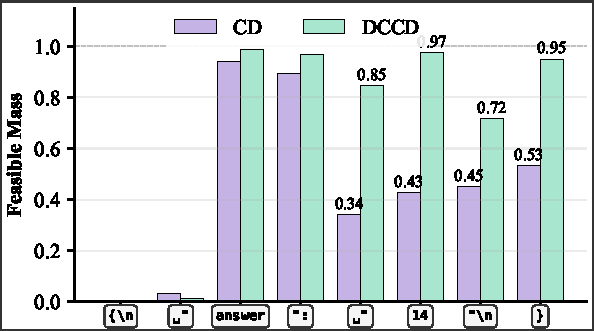
\includegraphics[width=\linewidth]{figs/cd_vs_dccd_icml.pdf}
\caption{\textbf{Low feasible mass results in distortion.}
Across tokens in a toy example, the feasible mass $\alpha(h_t)$ under constrained decoding is always $<0.53$ and is near zero for early tokens. In this setting, the constraint admits only $\approx 1\%$ of the full vocabulary as feasible tokens, forcing strong renormalization and accumulating KL distortion.}
    \label{fig:placeholder}
\end{figure}


\textbf{A toy example.} Consider a task whose output must be a single-slot JSON object of the form
$z=\texttt{\{"answer":}~a\texttt{\}}$, where $a\in\mathcal{V}_{\text{ans}}$ is a single semantic token.
The grammar forces a fixed sequence of formatting tokens $s_{1:m}$ (e.g., \texttt{\{}, quotes, field name, colon, delimiters),
followed by the semantic token $a$ at position $m{+}1$.
Thus, most decoding steps are formatting steps, and at many positions the valid-next-token set is a singleton.
If $A(h_t)=\{s_t\}$, constrained decoding deterministically emits $s_t$, and the renormalization factor is
$\alpha(h_t)=\pi_\theta(s_t\mid h_t)$.
When the base model would naturally respond in free-form text (e.g., ``The answer is 14.''), early schema tokens such as \texttt{`\{'} can have very low probability,
making $\alpha(h_t)$ small (see Figure \ref{fig:placeholder}) and the per-step distortion large.
Because the model is autoregressive, forcing a sequence of such low-probability formatting tokens drives generation through unlikely prefixes,
which can shift the model’s downstream distribution at the semantic slot $a$.

%

\textbf{Key challenge.}
In structured formats, low feasible mass often arises {not} because the model lacks the semantic solution, but because the schema enforces specific low-entropy tokens at specific times (quotes, delimiters, field names, operator symbols, etc.).
As a result, $\alpha(h_t)\ll 1$ can occur repeatedly across a generation (see Figure \ref{fig:placeholder}), causing constraint enforcement to accumulate substantial distortion and induce trajectory-dependent bias.
Empirically, this shows up as outputs that are perfectly well-formed yet semantically incorrect under strict constrained decoding~\citep{koo2024automata}.
This points to an actionable remedy: reduce distortion by {increasing feasible mass before enforcing constraints}, i.e., steer the model toward constraint-consistent continuations first, and only then apply hard token-level masking to retain exact validity guarantees.

\section{Draft-Conditioned Constrained Decoding}
\label{sec:method}
%
\begin{figure}[t]
    \centering
    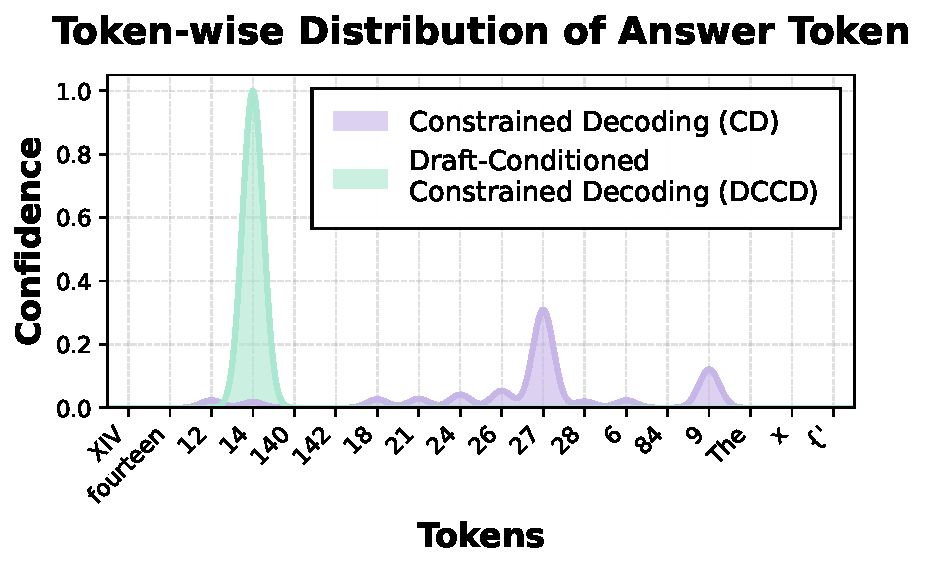
\includegraphics[width=\columnwidth]{figs/token_distribution_comparison.pdf}
    \caption{Token-wise confidence distribution for answer tokens in a single example. Constrained decoding spreads probability mass across multiple plausible answer tokens (``$6$'', ``$27$'', ``$28$'', ``$6$'', ``$84$'', ``$9$''), with the incorrect answer ``$27$'' receiving moderate confidence (0.46). DCCD shows a sharp, concentrated distribution with near-perfect confidence (1.0) on the correct token ``$14$''.}\label{fig:token_confidence}
\end{figure}
%
\subsection{Key insight: feasible mass is {context-dependent}}
\label{sec:key_insight}
%
Section~\ref{sec:problem} showed that the distortion induced by constrained decoding is governed by the feasible mass
\begin{align}
\alpha(h_t) \;=\; \sum_{a\in A(h_t)} \pi_{\theta}(a\mid h_t),
\end{align}
since
$\mathrm{KL}=\log \tfrac{1}{\alpha(h_t)}$ (cf. \eqref{eq:kl_log_alpha}).
At first glance, this suggests that at inference time, the model parameters are fixed, and the valid set
$A(h_t)$ is fixed by the schema/grammar. So what can we possibly change to make $\alpha(h_t)$ larger to reduce distortion? The key observation is that while $\pi_\theta$ is fixed, the {conditional distribution} is not, it depends on the
{conditioning context}.
In particular, if we append any auxiliary text $d$ (a ``draft'', ``plan'', or intermediate representation) to the context,
the model induces a {different} next-token distribution $\pi_\theta(a \mid h_t, d)$. This changes the feasible mass to
\begin{align}
\alpha(h_t; d)
\;\triangleq\;
\sum_{a\in A(h_t)} \pi_{\theta}(a\mid h_t, d).
\label{eq:alpha_with_d}
\end{align}
Thus, even though $A(h_t)$ is fixed, we can {increase the probability mass on valid tokens} by choosing an
appropriate auxiliary context $d$.
Our method will instantiate $d$ as an unconstrained draft generated by a language model, and then enforce the hard
constraint only after conditioning on this draft.
%
Now consider adding an auxiliary context $d$ that contains the intended content (e.g., a draft reasoning trace that ends with the correct answer).
Conditioning on $d$ changes the distribution over formatting tokens:
\begin{align}
\pi_\theta(s_t \mid h_t, d) \gg \pi_\theta(s_t \mid h_t)
 \Rightarrow
\alpha(h_t;d) \gg \alpha(h_t),
\end{align}
which reduces the projection tax at each forced formatting. As an example, an unconstrained response as auxiliary context can help improve the likelihood of a correct token, as shown in Figure \ref{fig:token_confidence}. 
Crucially, it also makes the forced prefix $s_{1:m}$ {in-distribution} under the conditioned model, so the answer-slot distribution
is better preserved.


\subsection{Proposed Algorithm}
\label{sec:two_stage}


Motivated by Eq.~\eqref{eq:alpha_with_d}, we implement the auxiliary context $d$ as an {unconstrained draft} $y$.
DCCD comprises of two autoregressive models:
a {draft model} $p_{\mathrm{draft}}$ for free-form planning and a {projector model} $p_{\mathrm{proj}}$ for structure-constrained generation.
They may be the same model ($p_{\mathrm{draft}}=p_{\mathrm{proj}}$), or $p_{\mathrm{proj}}$ could be smaller since this stage primarily performs structured realization.

\textbf{Step 1: Draft generation.}
We first sample a draft
\begin{align}
y \sim p_{\mathrm{draft}}(\cdot \mid x),
\label{eq:dccd_draft}
\end{align}
where $y$ can be a plan, an outline, or free-form reasoning and is \emph{not} required to satisfy the hard constraint.

\textbf{Step 2: Draft-conditioned constrained decoding.}
We then generate the final structured output $z_{1:T}$ using constrained decoding {conditioned on} $(x,y)$. We define
\begin{align}
p_2(z_t \mid \tilde h_t),
\qquad
\tilde h_t \triangleq (x, y, z_{<t}),
\label{eq:p2_def_rewrite}
\end{align}
where $p_2$ is instantiated by $p_{\mathrm{proj}}$ (which is $\pi_{\theta}$ in our case) with the draft $y$ included in context. 
The hard constraint still applies to the {final output prefix} $h_t=(x,z_{<t})$.
Therefore, the valid-next-token set remains $A(h_t)$ from Section~\ref{sec:problem}.
We enforce validity by masking and renormalizing under the conditioned distribution:
\begin{align}
\tilde q(z_t \mid \tilde h_t)
\;=\;
\frac{p_2(z_t\mid \tilde h_t)\,\mathbb{I}[z_t\in A(h_t)]}{\tilde\alpha(\tilde h_t)},
\label{eq:qtilde_rewrite}
\end{align}
with draft-conditioned feasible mass
\begin{align}
\tilde\alpha(\tilde h_t)\triangleq \sum_{a\in A(h_t)} p_2(a\mid \tilde h_t).
\label{eq:feasible_mass_tilde_rewrite}
\end{align}
We decode by sampling $z_t\sim \tilde q(\cdot\mid \tilde h_t)$ (or greedy decoding).

\textbf{Key connection to the challenge in Section~\ref{sec:problem}.}
Section~\ref{sec:problem} identified low feasible mass $\alpha(h_t)$ as the driver of projection tax and semantic distortion.
DCCD targets this directly: it seeks drafts $y$ such that $\tilde\alpha(\tilde h_t)\gg \alpha(h_t)$ along the realized trajectory.
In practice, the draft makes structural tokens (quotes, braces, delimiters, field names) much more probable, reducing repeated forced
``surprises'' and preserving the model's semantic preferences for the content tokens.
We summarize the proposed steps in Algorithm \ref{alg:dccd}. Algorithm~\ref{alg:dccd} presents DCCD in a general form that also subsumes several practical extensions.
In particular, the algorithm allows generating multiple unconstrained drafts in parallel ($K>1$) and selecting the final output via a late-selection criterion.
In our instantiation, we score each candidate using the cumulative log feasible mass incurred during constrained decoding, which directly reflects the amount of constraint-induced distortion.
However, the framework itself is agnostic to the specific selection rule: alternative criteria such as total log-likelihood under the constrained model, external verifier scores, task-specific judges, or majority voting across valid realizations can be substituted without changing the core procedure.
When $K=1$, DCCD reduces to a simple two-step draft-then-constrain decoding scheme.

\begin{algorithm}[t]
\caption{Draft-Conditioned Constrained Decoding}
\label{alg:dccd}
\begin{algorithmic}[1]
\REQUIRE Prompt $x$; draft model $p_{\mathrm{draft}}$; projector model $p_{\mathrm{proj}}$;
constraint oracle $A(\cdot)$; max length $T$; number of drafts $K$
\STATE Sample drafts $y^{(1)},\ldots,y^{(K)} \sim p_{\mathrm{draft}}(\cdot\mid x)$
\FOR{$k=1$ to $K$}
    \STATE $z^{(k)}_{<1}\leftarrow \emptyset$, \;\; $S^{(k)}\leftarrow 0$
    \FOR{$t=1$ to $T$}
        \STATE Compute $p_2(\cdot \mid x,y^{(k)},z^{(k)}_{<t})$ using $p_{\mathrm{proj}}$
        \STATE $\tilde\alpha_t^{(k)} \leftarrow \sum_{a\in A(x,z^{(k)}_{<t})} p_2(a \mid x,y^{(k)},z^{(k)}_{<t})$
        \STATE $S^{(k)} \leftarrow S^{(k)} + \log(\tilde\alpha_t^{(k)})$
        \STATE Form $\tilde q(\cdot)\propto p_2(\cdot)\odot \mathbb{I}[\cdot\in A(x,z^{(k)}_{<t})]$
        \STATE Sample (or greedily select) $z^{(k)}_{t} \sim \tilde q(\cdot)$
    \ENDFOR
\ENDFOR
\STATE Choose $k^\star \in \arg\max_k S^{(k)}$ (or $k^\star=1$ when $K{=}1$)
\STATE \textbf{return} $z^{(k^\star)}_{1:T}$
\end{algorithmic}
\end{algorithm}

\begin{figure*}[ht]
    \centering
    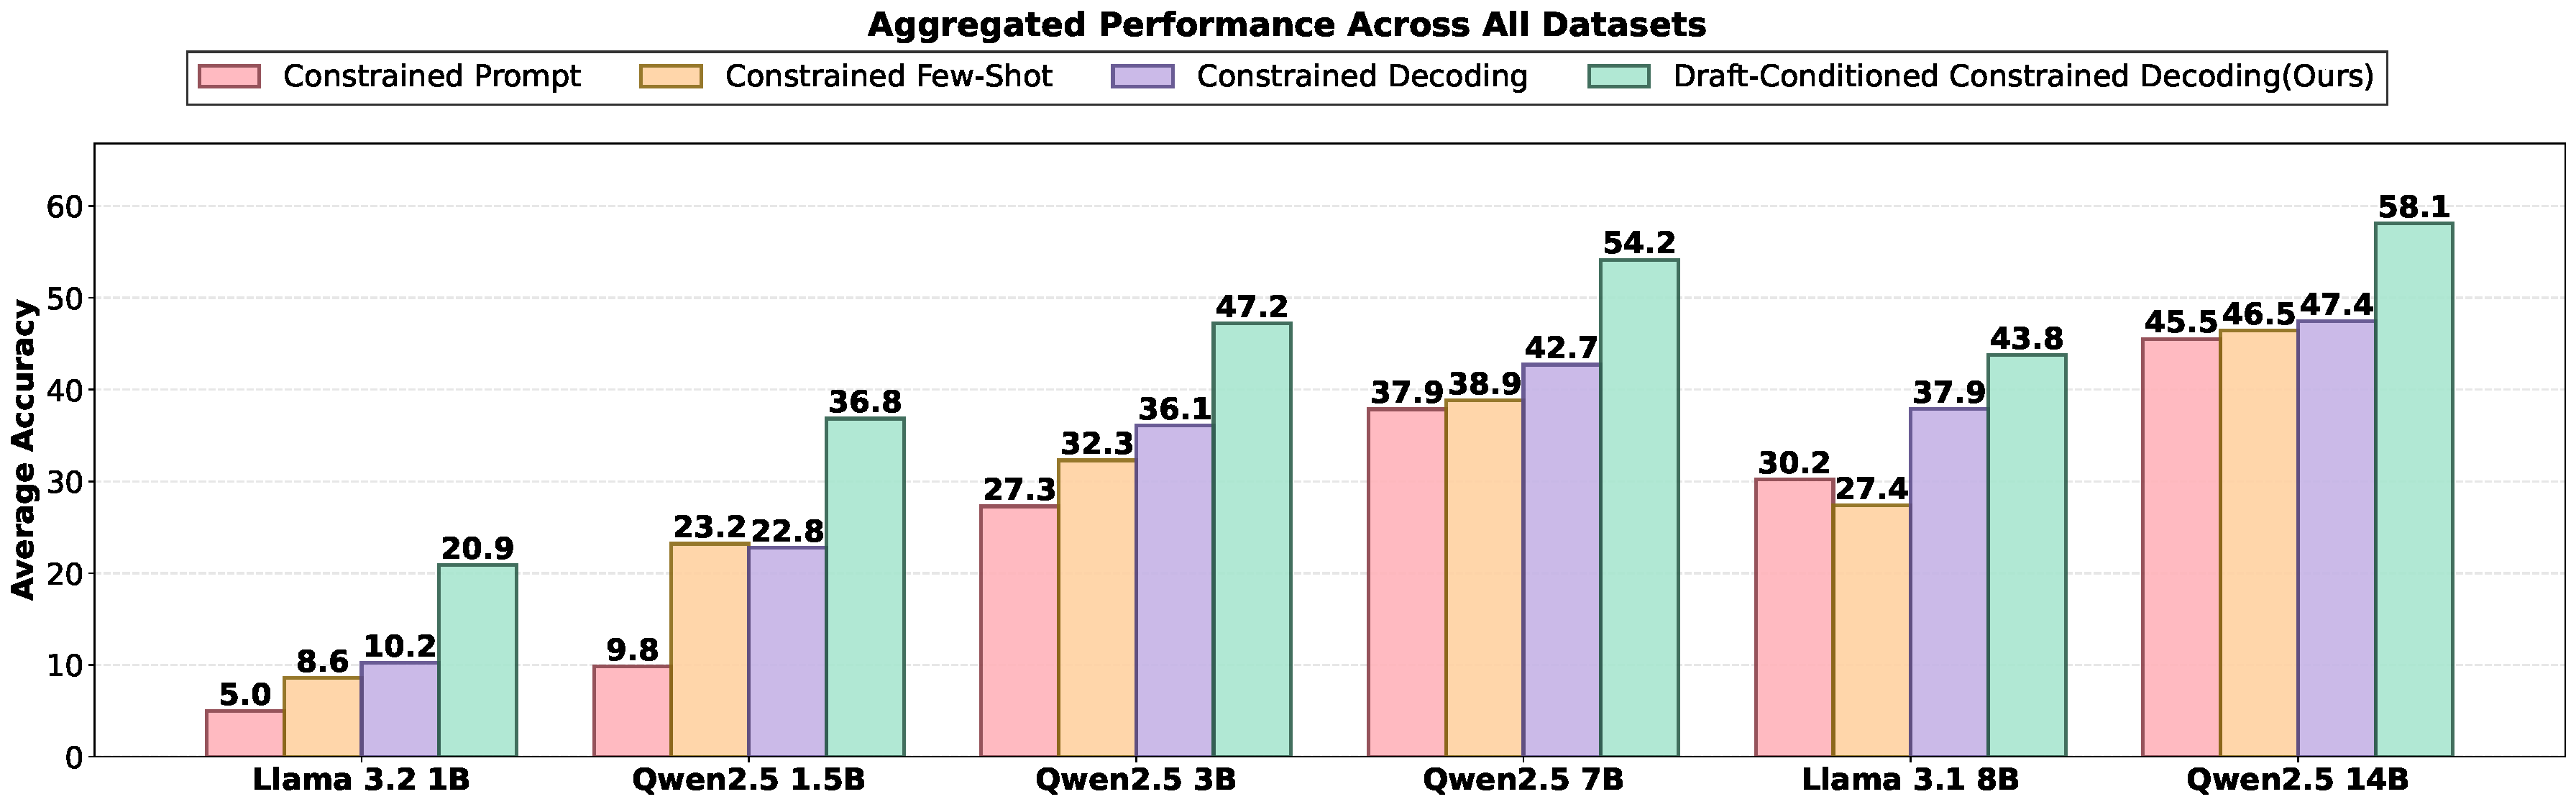
\includegraphics[width=\linewidth]{figs/aggregated_performance.pdf}
    \caption{\textbf{Average performance comparison across all evaluation datasets} (GSM8K, GSM Symbolic, Math500, and FOLIO). We compare prompting-based baselines (CP, CF), grammar-based constrained decoding (CD), and our
Draft-Conditioned Constrained Decoding (DCCD).
Across all model scales, DCCD achieves the best aggregated performance, with the largest relative gains for smaller models
where hard constraints induce the strongest projection distortion (e.g., 1B: 10.2$\%\rightarrow$20.9$\%$).
\textbf{Takeaway:} conditioning on an unconstrained draft before enforcing hard constraints yields consistent, model-agnostic improvements in strict structured generation.
}
    \label{fig:aggregated_performance}
\end{figure*}

\section{Experiments}
\label{sec:experiments}

We evaluate our proposed approach (DCCD) on structured generation tasks that require
both (i) {semantic correctness} and (ii) {exact structural validity}. Our experiments are designed to answer three questions:

 \textbf{Q1} (Effectiveness). Does DCCD improve {strict structured accuracy} compared to prompting-based methods and standard constrained decoding?
 
    \textbf{Q2} (Efficiency). Because DCCD composes two models, can it achieve better {parameter/cost efficiency} than single-model constrained decoding?
    
    \textbf{Q3} (Test-time scaling). How does DCCD scale with additional test-time compute (e.g., sampling $n$ candidates and voting/selecting)?



\subsection{Experimental Setup}
\label{sec:exp_setup}
\textbf{Datasets and structural constraints.}
We evaluate on GSM8K~\citep{cobbe2021training}, MATH500~\citep{hendrycksmath2021}, GSM-Symbolic~\citep{mirzadeh2024gsm}, and FOLIO~\citep{han2024p}, spanning numerical math, symbolic math,
and first-order logic formalization.
For each dataset, we enforce a strict, machine-checkable output format (JSON schemas, expression grammar, or FOL grammar),
with detailed examples of structures in Appendix \ref{app:dataset_examples}. (see Appendix \ref{additional_details} for more details).

\textbf{Models and baselines.}
We test instruction-tuned models\begin{wraptable}{r}{4cm}
\vspace{-10pt}
\caption{Models used}
\vspace{-6pt}
\centering
\setlength{\tabcolsep}{10pt}
\renewcommand{\arraystretch}{0.9}
\small
\begin{tabular}{@{}cc@{}}
\toprule
\textbf{Name} & \textbf{Model ID} \\
\midrule
14B & Qwen 2.5 14B \\
8B & Llama 3.1 8B \\
7B & Qwen 2.5 7B \\
3B & Qwen 2.5 3B \\
1.5B & Qwen 2.5 1.5B \\
1B & Llama 3.2 1B \\
\bottomrule
\end{tabular}
\vspace{-14pt}
\label{tab:models_cost_analysis}
\end{wraptable} ranging from 1B to 14B parameters (Table~\ref{tab:models_cost_analysis}). We compare against:
(i) {Constrained Prompting (CP)}\setlength{\columnsep}{2pt} and {Constrained Few-Shot (CF)} (prompt-only format enforcement),
and (ii) {Constrained Decoding (CD)} using XGrammar ~\citep{dong2025xgrammar}, which guarantees structural validity by masking invalid tokens.


\textbf{Evaluation metric.}
Our evaluation framework assesses two aspects of the response:   (i) {answer correctness}  by comparing the model's final answer against the ground truth, and (ii) structural compliance by verifying that the output strictly adheres to the specified format constraints (JSON schema for mathematical tasks, logical formalism for FOLIO). Then, a response is marked as successful only when \textit{both} conditions are satisfied. This joint evaluation captures the core challenge of structured generation: maintaining reasoning quality while satisfying hard constraints.

\subsection{Main Results}
\label{sec:exp_results}

\begin{table}[H]
\centering
%\small
\caption{
Comparison of constrained decoding strategies across datasets. {CP:} Constrained Prompting, {CF:} Constrained Few Shot,\textbf{ CD:}  Constrained Decoding, {DCCD:} Draft Conditioned Constrained Decoding.
}
\label{tab:stage_comparison_with_prompt}
\resizebox{\columnwidth}{!}{
\begin{tabular}{cccccc}
\toprule
& & \multicolumn{4}{c}{\textbf{Datasets}} \\
\cmidrule(lr){3-6}
\textbf{Model Size} 
& \textbf{Algorithm}
& \textbf{GSM8K}
& \textbf{GSM Symbolic}
& \textbf{Math500}
& \textbf{FOLIO}
\\
\midrule
% ------------------ Llama 3.2 1B ------------------
\multirow{4}{*}{\textbf{1B}}
& CP
& 7.51 & 6.00 & 6.40 & 0.00 \\
& CF
& 13.80 & 9.00 & 11.60 & 0.00 \\
& CD
& 15.24 & 0.00 & 6.00 & 19.70 \\
\cellcolor{white}  &  \cellcolor{lightblue}   DCCD (ours) 
& \cellcolor{lightblue}  \textbf{39.04} & \cellcolor{lightblue}  \textbf{9.00} & \cellcolor{lightblue}  \textbf{19.80} & \cellcolor{lightblue}  \textbf{21.67} \\
\midrule
% ------------------ Qwen 2.5 1.5B ------------------
\multirow{4}{*}{\textbf{1.5B}}
& CP
& 13.27 & 11.00 & 15.00 & 0.00 \\
& CF
& 48.22 & 23.00 & 21.60 & 0.00 \\
& CD
& 49.36 & 12.00 & 15.00 & 14.78 \\
\cellcolor{white}  & \cellcolor{lightblue}  DCCD (ours)
&  \cellcolor{lightblue}  \textcolor{black}{\textbf{73.92}} & \cellcolor{lightblue}  \textcolor{black}{\textbf{23.00}} & \cellcolor{lightblue}  \textcolor{black}{\textbf{38.20}} &  \cellcolor{lightblue}  \textcolor{black}{\textbf{18.23}} \\
\midrule
% ------------------ Qwen 2.5 3B ------------------
\multirow{4}{*}{\textbf{3B}}
& CP
& 59.14 & 19.00 & 30.00 & 1.00 \\
& CF
& 71.80 & 25.00 & 32.40 & 0.00 \\
& CD
& 73.24 & 17.00 & 33.40 & 20.69 \\
\cellcolor{white} & \cellcolor{lightblue}  DCCD (ours)
&  \cellcolor{lightblue}  \textcolor{black}{\textbf{84.53}} & \cellcolor{lightblue}  \textcolor{black}{\textbf{36.00}} &  \cellcolor{lightblue}  \textcolor{black}{\textbf{46.80}} &  \cellcolor{lightblue}  \textcolor{black}{\textbf{21.67}} \\
\midrule
% ------------------ Qwen 2.5 7B ------------------
\multirow{4}{*}{\textbf{7B}}
& CP
& 80.06 & 31.00 & 40.40 & 0.00 \\
& CF
& 82.26 & 29.00 & 44.20 & 0.00 \\
& CD
& 81.58 & 26.00 & 43.60 & 19.70 \\
\cellcolor{white}  & \cellcolor{lightblue} DCCD (ours)
& \cellcolor{lightblue} \textcolor{black}{\textbf{91.28}} & \cellcolor{lightblue}\textcolor{black}{\textbf{41.00}} & \cellcolor{lightblue}\textcolor{black}{\textbf{52.80}} & \cellcolor{lightblue}\textcolor{black}{\textbf{31.53}} \\
\midrule
% ------------------ Llama 3.1 8B ------------------
\multirow{4}{*}{\textbf{8B}}
& CP
& 76.80 & 17.00 & 27.00 & 0.00 \\
& CF
& 70.20 & 14.00 & 24.80 & 0.49 \\
& CD
& 80.89 & 19.00 & 28.60 & 23.15 \\
\cellcolor{white}  &\cellcolor{lightblue} DCCD (ours)
& \cellcolor{lightblue} \textcolor{black}{\textbf{83.02}} & \cellcolor{lightblue}\textcolor{black}{\textbf{30.00}} & \cellcolor{lightblue}\textcolor{black}{\textbf{35.00}} & \cellcolor{lightblue}\textcolor{black}{\textbf{27.09}} \\
\midrule
% ------------------ Qwen 2.5 14B ------------------
\multirow{4}{*}{\textbf{14B}}
& CP
& 91.13 & 44.00 & 47.00 & 0.00 \\
& CF
& 90.52 & 49.00 & 45.80 & 0.49 \\
& CD
& 86.43 & 37.00 & 47.60 & 18.72 \\
\cellcolor{white}  &\cellcolor{lightblue} DCCD (ours)
& \cellcolor{lightblue}\textbf{95.15} & \cellcolor{lightblue}\textbf{53.00} & \cellcolor{lightblue}\textbf{58.60}& \cellcolor{lightblue} \textbf{25.62} \\
\bottomrule
\end{tabular}}
\vspace{2pt}
\end{table}


\begin{figure*}[ht]
    \centering
    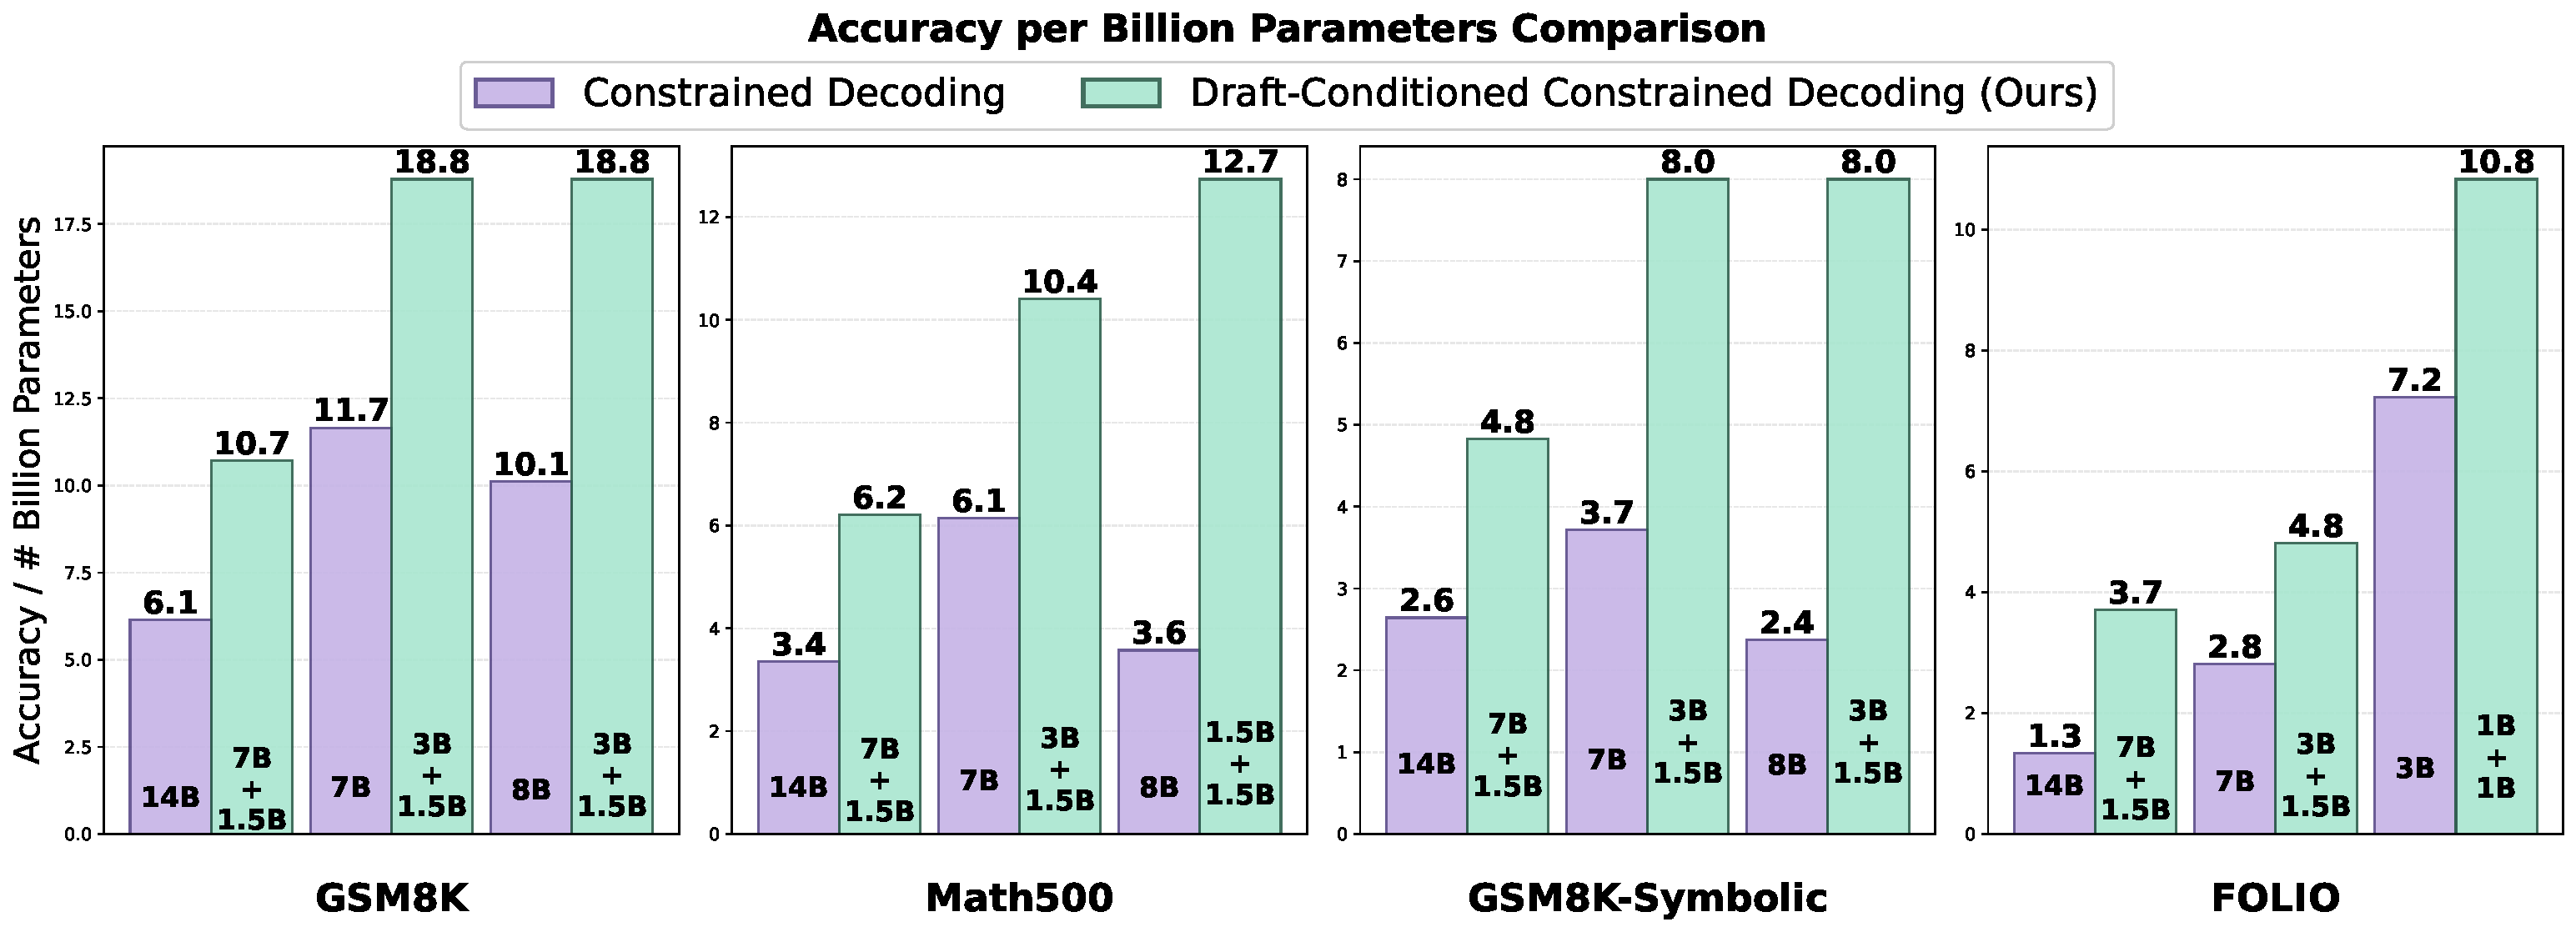
\includegraphics[width=\linewidth]{figs/accuracy_per_billion_parameters_comparison.pdf}
    \caption{\textbf{Parameter efficiency (accuracy per billion parameters).}
For each dataset, we report strict structured accuracy normalized by total parameters for single-model CD and parameter-matched DCCD compositions.
DCCD consistently achieves higher accuracy per parameter, with the largest gains in low-capacity regimes.}

    \label{fig:efficiency_comparison}
\end{figure*}

\textbf{\textbf{A1: DCCD improves strict structured accuracy across model scales and constraint types.}}
Figure~\ref{fig:aggregated_performance} summarizes the main result: when we average strict accuracy across all benchmarks,
DCCD consistently outperforms constrained prompting (CP), constrained few-shot (CF), and standard constrained decoding (CD)
for every model scale from 1B to 14B.
Table~\ref{tab:stage_comparison_with_prompt} then breaks this aggregate view into per-dataset results, showing that the gains
hold across heterogeneous constraint types (JSON schemas, expression grammars, and prover-checked logical forms).
Overall, DCCD delivers the best performance in all model–dataset configurations, with particularly large improvements
for smaller models, which is consistent with our projection-tax view that draft conditioning increases feasible mass before masking and
thereby reduces constraint-induced distortion. \\
\textbf{Takeaway:} DCCD is a training-free decoding strategy that reliably boosts {strict} structured generation accuracy across
models and constraint types, with particularly large benefits in the low-parameter regime where constrained decoding is most distortive.


\textbf{\textbf{A2: DCCD enables parameter-efficient model composition.}}
Figure~\ref{fig:efficiency_comparison} compares {accuracy per billion parameters} across all four benchmarks,
highlighting how effectively each method uses model capacity.
Across GSM8K, MATH500, GSM-Symbolic, and FOLIO, DCCD consistently achieves substantially higher accuracy per parameter
than single-model constrained decoding, often by large margins.
The gains are especially pronounced in low- to mid-capacity regimes: for example, on MATH500,
a $1.5\text{B}+1.5\text{B}$ DCCD composition (3B total) achieves {12.7} accuracy per billion parameters,
compared to {3.6} for an 8B model using constrained decoding, which is a {253\% efficiency improvement}.
Similarly, on GSM8K, a $7\text{B}+1.5\text{B}$ composition (8.5B total) outperforms a single 14B model
(10.7 vs.\ 6.1 accuracy per billion), despite using {39\% fewer parameters}.
%
This pattern holds consistently across tasks and scales, indicating that DCCD does not only shift performance,
but fundamentally improves how parameters are utilized.\\
\textbf{Takeaway.} DCCD enables smaller, cheaper model pairs to match or exceed much larger constrained baselines,
demonstrating that separating reasoning from formatting yields substantial gains in parameter efficiency.
%
\begin{figure}[t]
    \centering
    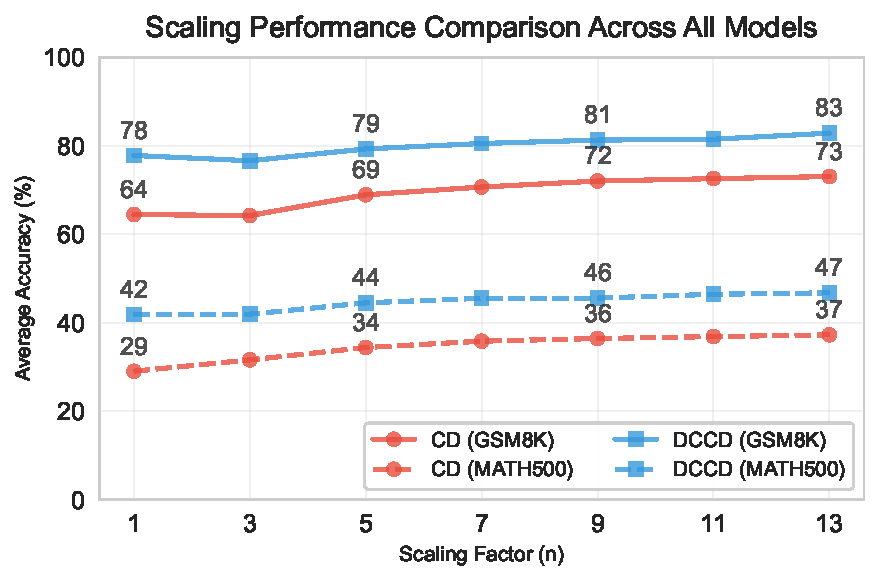
\includegraphics[width=\columnwidth]{figs/scaling_averaged_accuracy_both_benchmarks.pdf}
    \caption{\textbf{Test-time scaling comparison} across GSM8K and MATH500 (averaged over six models, 1.5B-14B parameters). Solid lines: GSM8K; dashed lines: MATH500. Draft-Conditioned Constrained Decoding (blue) shows superior scaling versus Constrained Decoding (red), with widening performance gaps as n increases from 1 to 13.}
    \label{fig:scaling_comparison}
\end{figure}

\textbf{\textbf{A3: DCCD scales better with test-time sampling than constrained decoding.}}
We evaluate test-time scaling by sampling $n\in\{1,3,5,7,9,11,13\}$ candidates and applying majority vote at inference time.
For constrained decoding (CD), we vote over $n$ independently generated \emph{structured} outputs.
For DCCD, we vote over $n$ unconstrained \emph{drafts} (Stage~1) and then run a single constrained projection (Stage~2) on the selected draft.
Figure~\ref{fig:scaling_comparison} shows that DCCD benefits more from additional test-time compute on both benchmarks.
On GSM8K, DCCD improves from 78\% at $n{=}1$ to 83\% at $n{=}13$, while CD improves from 64\% to 73\%. 
\begin{figure}[t]
    \centering
    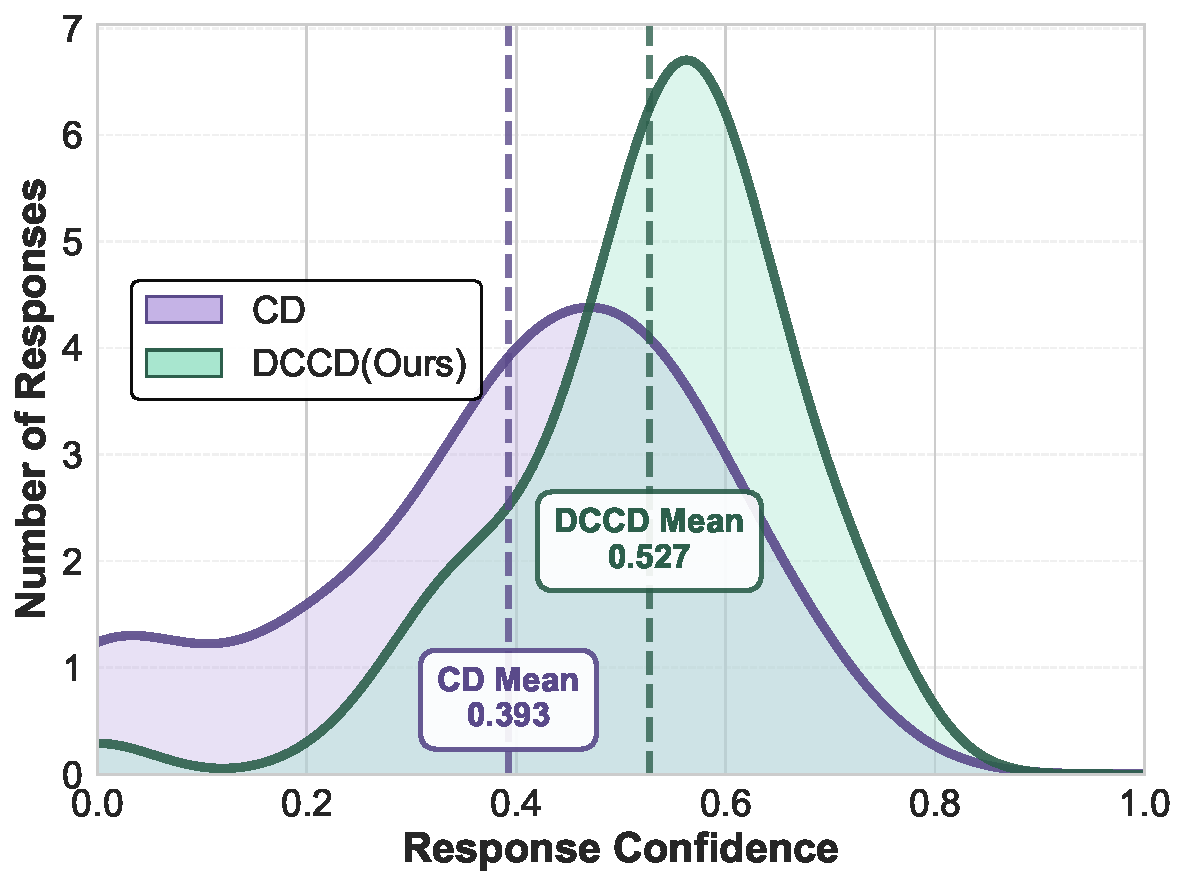
\includegraphics[width=\linewidth]{figs/cd_vs_joint_probability_comparison_kde_only.pdf}
    \caption{Distribution of response confidence scores for Llama 3.2 3B Instruct on GSM8K. The histogram compares the confidence distributions between standard Constrained Decoding (CD) using $q(y|x)$ and Draft-Conditioned Constrained Decoding (DCCD) using joint probability $p_{\text{draft}}(d|x) \cdot p_2(y|x,d)$. DCCD demonstrates a significant rightward shift with mean confidence of 0.527 compared to CD's 0.393, indicating 39\% higher confidence in generated responses. }
    \label{fig:response_confidence}
\end{figure}
On MATH500, DCCD improves from 42\% to 47\% whereas CD improves from 29\% to 37\%, and the performance gap remains large throughout.
In both cases, gains saturate beyond moderate $n$ (around $n\approx 7$), suggesting diminishing returns once the best drafts/solutions are already sampled.

\textbf{Takeaway:} Allocating test-time compute to sampling diverse \emph{drafts} (semantic plans) is more effective than repeatedly sampling under hard constraints, and DCCD converts this additional compute into higher structured accuracy.


\subsection{Additional Insights}
\textbf{Response-Level Confidence.} We compared the response-level confidence of Llama 3.2 3B Instruct on the GSM8K dataset. Figure \ref{fig:response_confidence} shows the distribution of response probability confidence scores. We evaluated the final response confidence of CD as $q(y|x)$ and the joint probability of the draft and draft-conditioned final response in DCCD as $p_{\text{draft}}(d|x) \cdot p_2(y|x,d)$. DCCD elicited responses with 39\% higher confidence compared to CD, which directly contributed to improved strict accuracy on the dataset.

\textbf{Non-Verifiable Tasks.} We designed an additional experiment to assess the robustness of DCCD on tasks without ground-truth verification. The objective was to generate 256-token TL;DR summaries across various topics (see Appendix \ref{non-verifiable} for details). We evaluated DCCD and CD responses using win rate percentage across three criteria: overall quality, faithfulness, and coverage. Figure \ref{fig:win-rate-unverifiable} demonstrates that DCCD achieves approximately 80\% win rate over CD across all evaluation categories. This finding supports our hypothesis that for reasoning-intensive tasks, a staged inference procedure is preferable to direct generation.
%
\begin{figure}[t]
    \centering
    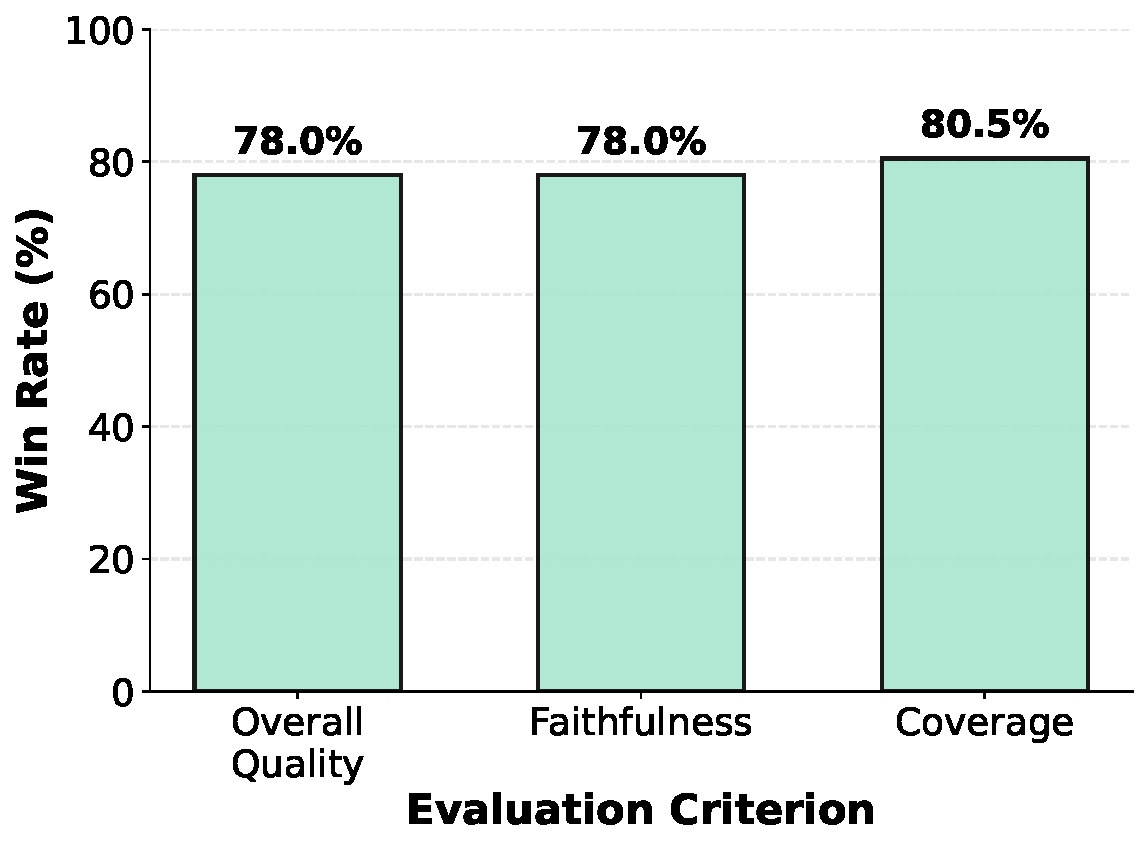
\includegraphics[width=\columnwidth]{figs/dccd_winrate.pdf}
    \caption{Win rate comparison between DCCD and CD on non-verifiable summarization tasks. LLM as a Judge assessed 256-token TL;DR summaries across three criteria: overall quality, faithfulness, and coverage. DCCD consistently outperforms CD with approximately 78--80.5\% win rate across all evaluation dimensions, demonstrating the effectiveness of staged inference for reasoning-intensive generation tasks.}
    \label{fig:win-rate-unverifiable}
\end{figure}
%

\section{Conclusion}
\label{sec:conclusion}
%
We studied structured generation under hard constraints, where outputs must be both semantically correct and strictly valid
(e.g., JSON schemas, expression grammars, and prover-checked logical forms). We showed that standard constrained decoding
can be interpreted as repeated reverse-KL projections onto a prefix-valid set, and that its quality degradation is driven by low
probability mass on valid continuations, incurring a cumulative ``projection tax'' and trajectory bias. Motivated by this view, we
proposed {Draft-Conditioned Constrained Decoding (DCCD)}, a training-free two-stage inference procedure that first
generates an unconstrained draft (semantic plan) and then performs constrained decoding conditioned on the draft, increasing
valid mass \emph{before} projection while retaining exact validity guarantees. Across GSM8K variants, MATH500, and
FOLIO/Prover9 and model scales from 1B to 14B, DCCD consistently improves strict structured accuracy, enables
parameter-efficient model composition, and converts additional test-time compute into larger gains than standard constrained
decoding. Overall, {decoupling semantic planning from structural enforcement} is a simple, effective recipe for reliable
structured generation.

\section*{Impact Statement}

This paper presents work whose goal is to advance the field of machine learning by improving the reliability of structured generation in large language models. While the proposed method may support more robust deployment of LLMs in software and tool-based systems, we do not foresee any new or unique societal risks beyond those already associated with large language models. We believe no additional ethical considerations are required beyond existing best practices for responsible AI deployment.

% \nocite{langley00}

\bibliography{example_paper}
\bibliographystyle{icml2026}

%%%%%%%%%%%%%%%%%%%%%%%%%%%%%%%%%%%%%%%%%%%%%%%%%%%%%%%%%%%%%%%%%%%%%%%%%%%%%%%
%%%%%%%%%%%%%%%%%%%%%%%%%%%%%%%%%%%%%%%%%%%%%%%%%%%%%%%%%%%%%%%%%%%%%%%%%%%%%%%
% APPENDIX
%%%%%%%%%%%%%%%%%%%%%%%%%%%%%%%%%%%%%%%%%%%%%%%%%%%%%%%%%%%%%%%%%%%%%%%%%%%%%%%
%%%%%%%%%%%%%%%%%%%%%%%%%%%%%%%%%%%%%%%%%%%%%%%%%%%%%%%%%%%%%%%%%%%%%%%%%%%%%%%
\clearpage
\onecolumn
\icmltitle{Appendix}
\tableofcontents
\clearpage
\appendix
\section{{Why a larger feasible mass can improve accuracy}}
\label{sec:why_accuracy}

The toy example builds intuition, but we can also give a simple \emph{distributional stability} justification.

Let $U(x,z)\in[0,1]$ be any bounded utility, and define the \emph{validity-gated} utility
\begin{align}
\bar U(x,z) \;\triangleq\; U(x,z)\,\mathbb{I}[z\in\mathcal{L}(x)].
\end{align}
This makes invalid strings automatically receive zero utility, matching strict evaluation.

For any two sequence distributions $P$ and $Q$ over $\mathcal{V}^\star$,
\begin{align}
\big|\mathbb{E}_{z\sim P}[\bar U(x,z)] - \mathbb{E}_{z\sim Q}[\bar U(x,z)]\big|
\;\le\;
\mathrm{TV}(P,Q)
\;\le\;
\sqrt{\tfrac{1}{2}\mathrm{KL}(P\|Q)},
\label{eq:pinsker}
\end{align}
where the second inequality is Pinsker's inequality.
Therefore, whenever constrained decoding yields a distribution $P$ that is \emph{close in KL} to a reference distribution $Q$
that already assigns high utility to valid outputs, the constrained procedure cannot lose too much utility.

In our setting, standard constrained decoding defines $P=\rho_q(\cdot\mid x)$ and $Q=\rho_\theta(\cdot\mid x)$, and
Section~\ref{sec:problem} shows
\begin{align}
\mathrm{KL}\!\left(\rho_q(\cdot\mid x)\,\|\,\rho_\theta(\cdot\mid x)\right)
=
\mathbb{E}_{z\sim \rho_q(\cdot\mid x)}\Bigg[\sum_{t=1}^T \log\frac{1}{\alpha(h_t)}\Bigg].
\end{align}
Thus, increasing feasible mass $\alpha(h_t)$ (especially on prefixes actually visited during decoding) directly reduces the KL term,
which tightens the worst-case utility degradation bound in Eq.~\eqref{eq:pinsker}.
This provides a principled reason that ``making valid tokens higher-likelihood'' can translate into higher strict accuracy:
it reduces the amount by which the constraint mechanism can perturb the model away from its high-utility behavior.


\section{Additional details of experiments}
\label{additional_details}

\textbf{Datasets}
We evaluate on four datasets spanning numerical mathematical reasoning, symbolic mathematical reasoning, and logical deduction:

\begin{enumerate}[leftmargin=4mm, itemsep=1pt, topsep=2pt, parsep=0pt, partopsep=0pt]

\item \textbf{Numerical Math} We evaluate on three math datasets: \textbf{GSM8K}~\citep{cobbe2021training}, comprising grade school math word problems requiring multi-step arithmetic reasoning; \textbf{MATH500}~\citep{hendrycksmath2021}, a subset of 500 problems from the MATH benchmark covering algebra, geometry, and number theory.


\item \textbf{Symbolic Math.} \textbf{GSM-Symbolic}~\citep{mirzadeh2024gsm}, a symbolic variant of GSM8K designed to test genuine mathematical reasoning rather than pattern matching.

\item \textbf{Logical Reasoning.} \textbf{FOLIO}~\citep{han2024p}, a first-order logic reasoning dataset requiring structured logical formalization. Given natural language premises and a conclusion, models must produce a formal representation. Outputs are verified using the Prover9 theorem, and accuracy is measured by whether the formalized proof matches the ground truth conclusion.

\end{enumerate}


\textbf{Baselines}
We compare DCCD three established approaches for structured generation, which fall into two categories based on their primary strengths:

\begin{enumerate}[leftmargin=4mm, itemsep=1pt, topsep=2pt, parsep=0pt, partopsep=0pt]
    \item[] The below methods prioritize generating correct answers but struggle with strict format adherence:
    \item \textbf{Constrained Prompting(CP)} : System prompts are carefully engineered to specify the required output structure, including explicit format constraints and examples of valid outputs.
    
    \item \textbf{Constrained Few-Shot (CF)}: In addition to format specifications, we provide $k = 3$ in-context examples that demonstrate the expected output structure, following standard few-shot prompting practices.
    
    \vspace{3pt}
    \item[] This below method guarantees format compliance but often sacrifices answer quality:
    \item \textbf{Constrained Decoding (CD)}: We employ grammar-based constrained decoding using XGrammar~\citep{dong2025xgrammar} integrated with vLLM. At each decoding step, a token mask is constructed from the grammar specification, restricting sampling exclusively to syntactically valid tokens. This approach guarantees syntactic correctness but directly intervenes in the generation process, potentially limiting the model's reasoning capabilities.
\end{enumerate}


\section{Probability of the Token Positions}

\begin{figure}[H]
    \centering
    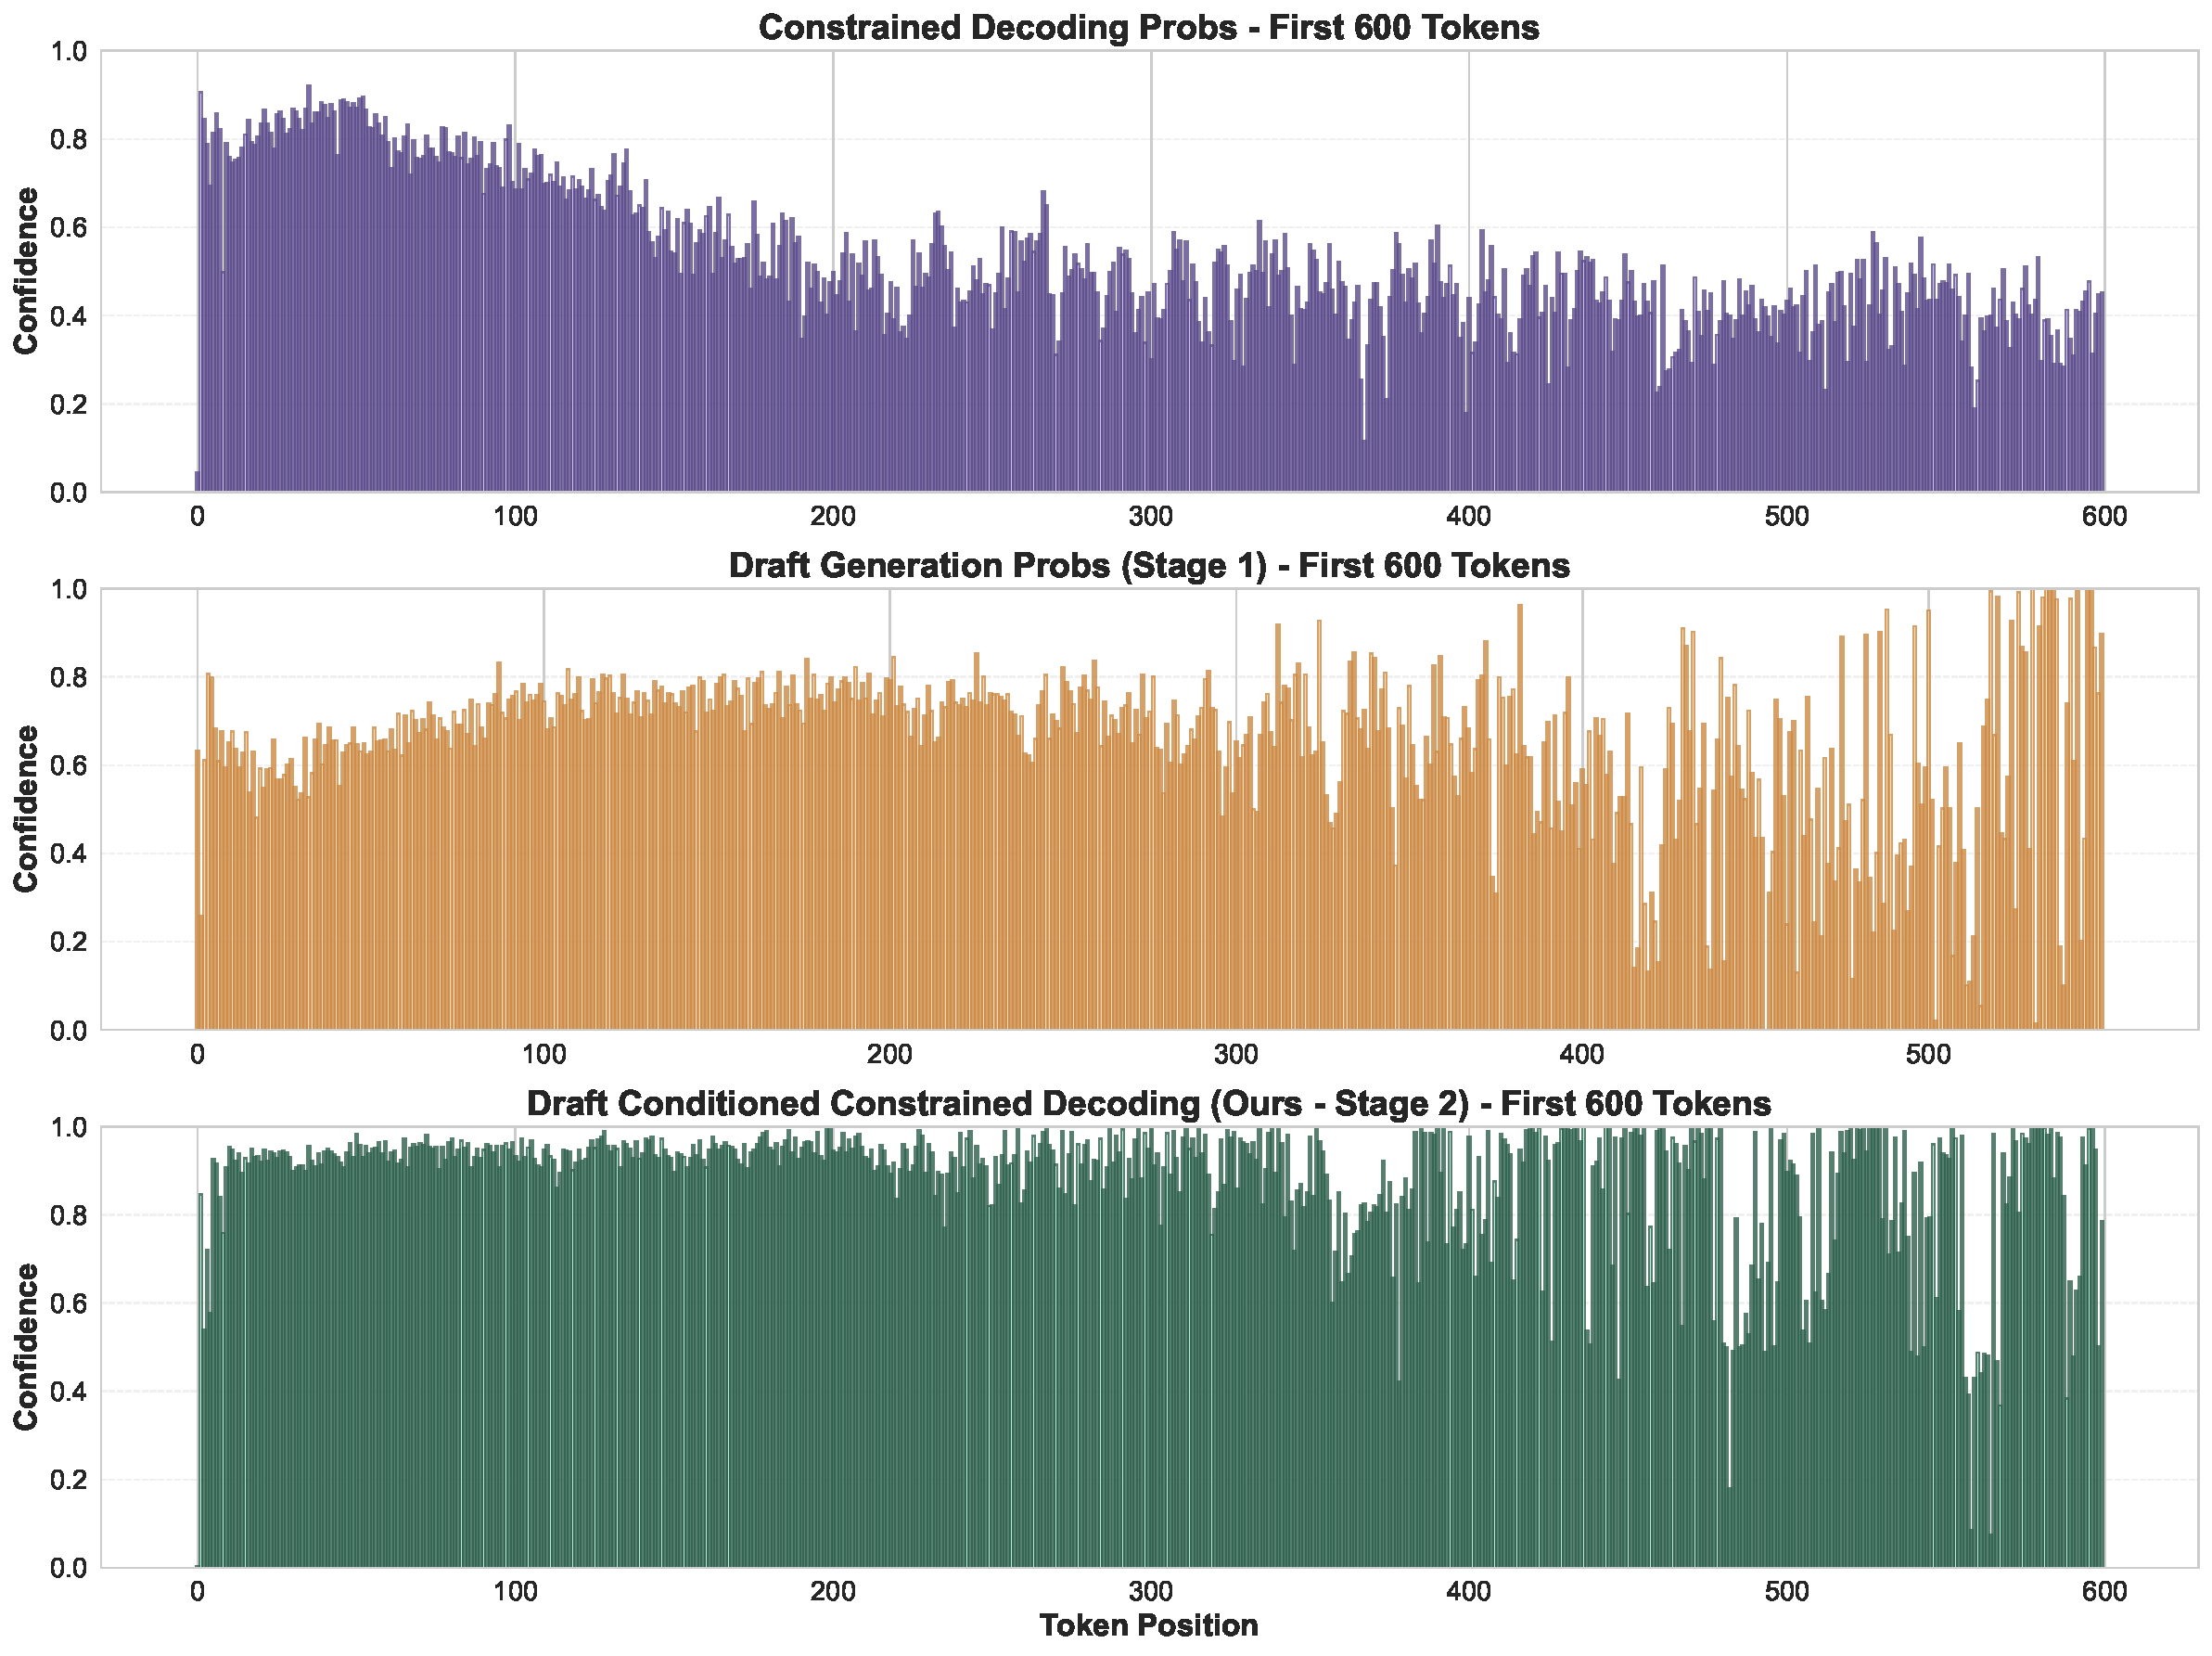
\includegraphics[width=0.8\linewidth]{figs/normalized_prob_by_position_bars_zoomed.pdf}
    \caption{Token-wise probability distributions across the first 600 token positions for different decoding strategies. Constrained Decoding (top) shows degraded confidence over longer sequences, with probabilities declining from 0.8 initially to 0.35 in later positions. Draft Generation (middle) maintains consistent moderate probabilities throughout without structural constraints. Draft-Conditioned Constrained Decoding (bottom, ours) sustains high confidence  across all positions, demonstrating that our Draft-Conditioned Constrained Decoding approach successfully maintains model confidence while enforcing structural constraints.}
    \label{fig:token_position_probs}
\end{figure}


\begin{figure}[h]
    \centering
    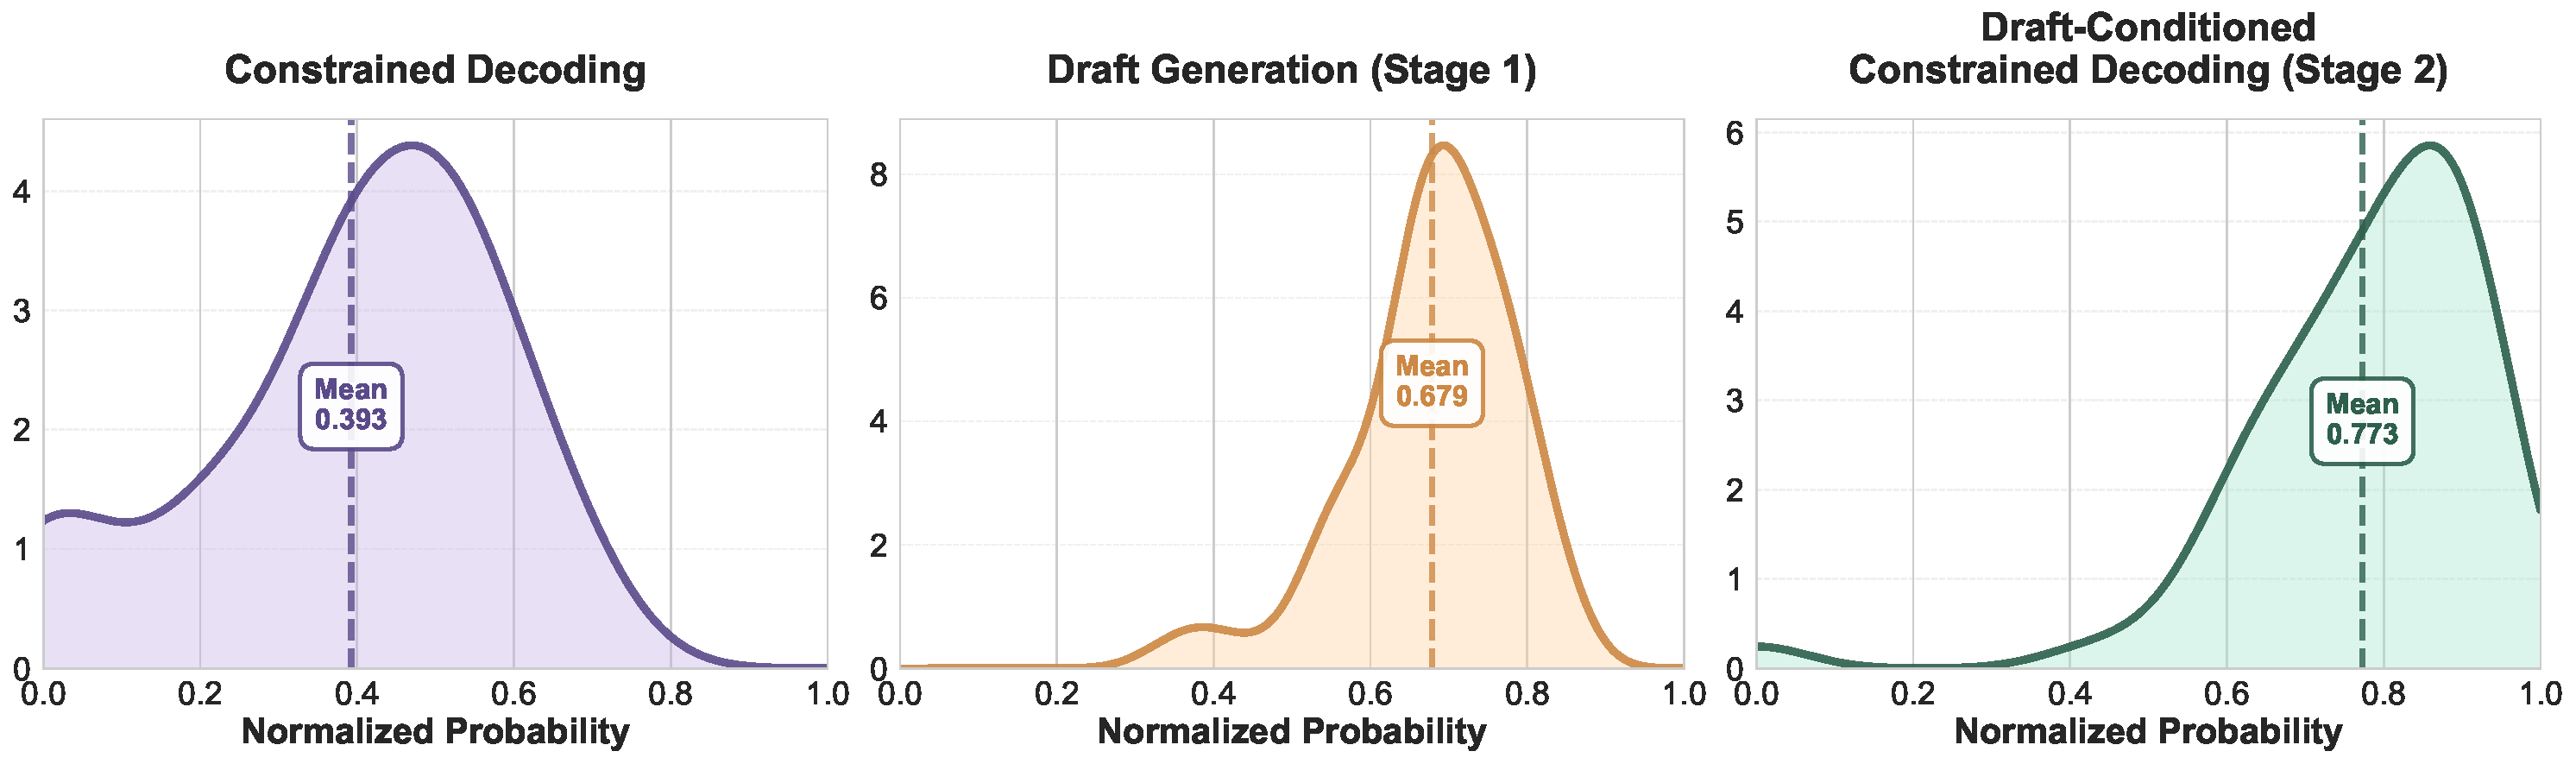
\includegraphics[width=\linewidth]{figs/normalized_response_prob_kde_only.pdf}
    \label{fig:normalized_prob_dist}
    \caption{Probability distribution analysis across decoding strategies. (a) Normalized token-level probability distributions show that Draft-Conditioned Constrained Decoding (DCCD, Stage 2) achieves significantly higher mean probability (0.527) compared to Constrained Decoding (CD, 0.393), indicating improved model confidence. Draft Generation (Stage 1) serves as the intermediate unconstrained reasoning step. (b) Comparison between  CD and DCCD Joint Probability (product of Stage 1 and Stage 2). Despite combining two probabilistic stages, the DCCD approach maintains substantially higher mean probability (0.527 vs 0.393), demonstrating that separating reasoning from formatting preserves model confidence while achieving structural constraints.}
    \label{fig:probability_analysis}
\end{figure}

\section{Test Time Scaling: Detailed Results}

Figure~\ref{fig:scaling_detailed} presents the complete test-time scaling results for all six models on both GSM8K and MATH500 benchmarks. These detailed breakdowns complement the aggregated results shown in Figure~\ref{fig:scaling_comparison} of the main paper.

Across all model sizes, we observe consistent patterns: 1) Draft-Conditioned Constrained Decoding(DCCD)(blue) consistently outperforms Constrained Decoding (red) at every scaling factor. 2) Smaller models (Llama 3.2 1B, Qwen2.5 1.5B) show larger absolute performance gaps, with Two-Stage Decoding maintaining significantly higher accuracy even at n=1. 3) Larger models (Qwen2.5 14B, Llama 3.1 8B, Qwen2.5 7B) demonstrate strong baseline performance with DCCD , approaching or exceeding 90\% on GSM8K. 4) On the more challenging MATH500 benchmark, the scaling behavior is more gradual, with performance improvements continuing through n=13, though at diminishing rates. 5) Constrained Decoding exhibits more pronounced degradation on smaller models, particularly evident in the Llama 3.2 1B results where accuracy remains below 15\% across all scaling factors on GSM8K.

The individual model trajectories reveal that the separation of reasoning from formatting provides consistent advantages across the entire model size spectrum, validating our approach's robustness and general applicability.

\begin{figure*}[h!]
    \centering
    \begin{subfigure}[b]{\textwidth}
        \centering
        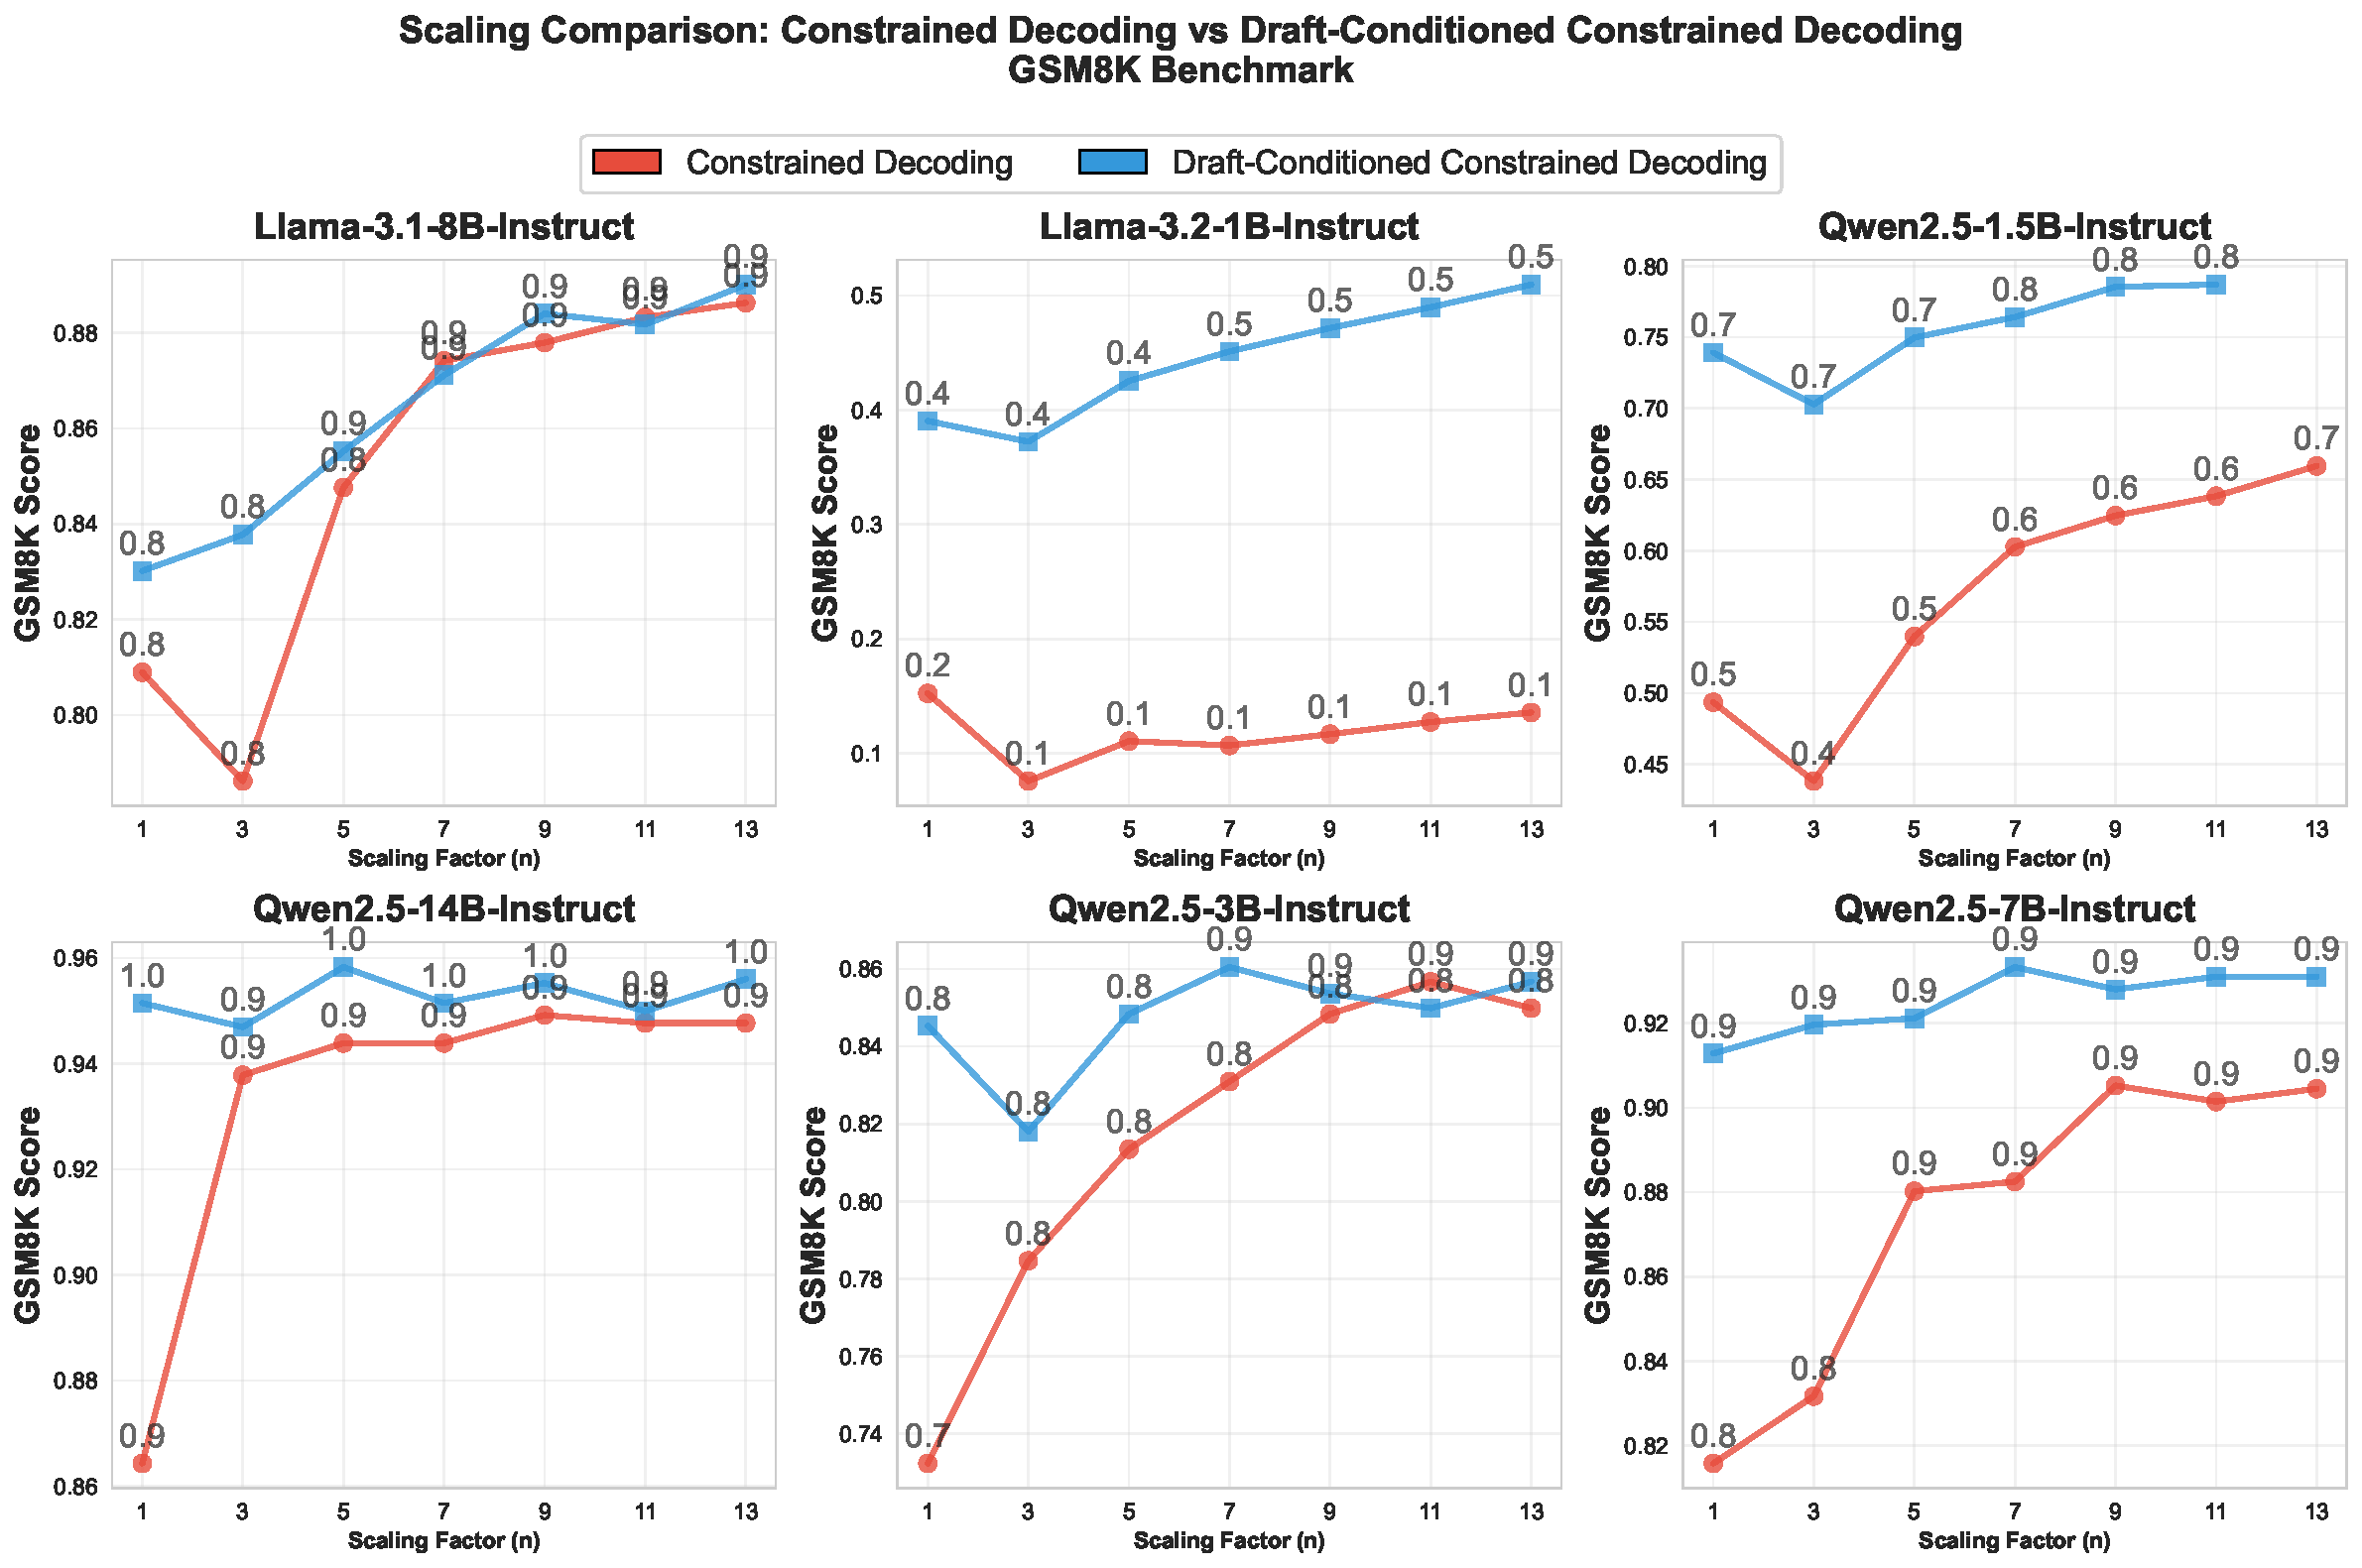
\includegraphics[width=0.9\linewidth]{figs/scaling_comparison_gsm8k.pdf}
        \caption{GSM8K benchmark scaling results}
        \label{fig:scaling_gsm8k_detailed}
    \end{subfigure}
    
    \vspace{0.5cm}
    
    \begin{subfigure}[b]{\textwidth}
        \centering
        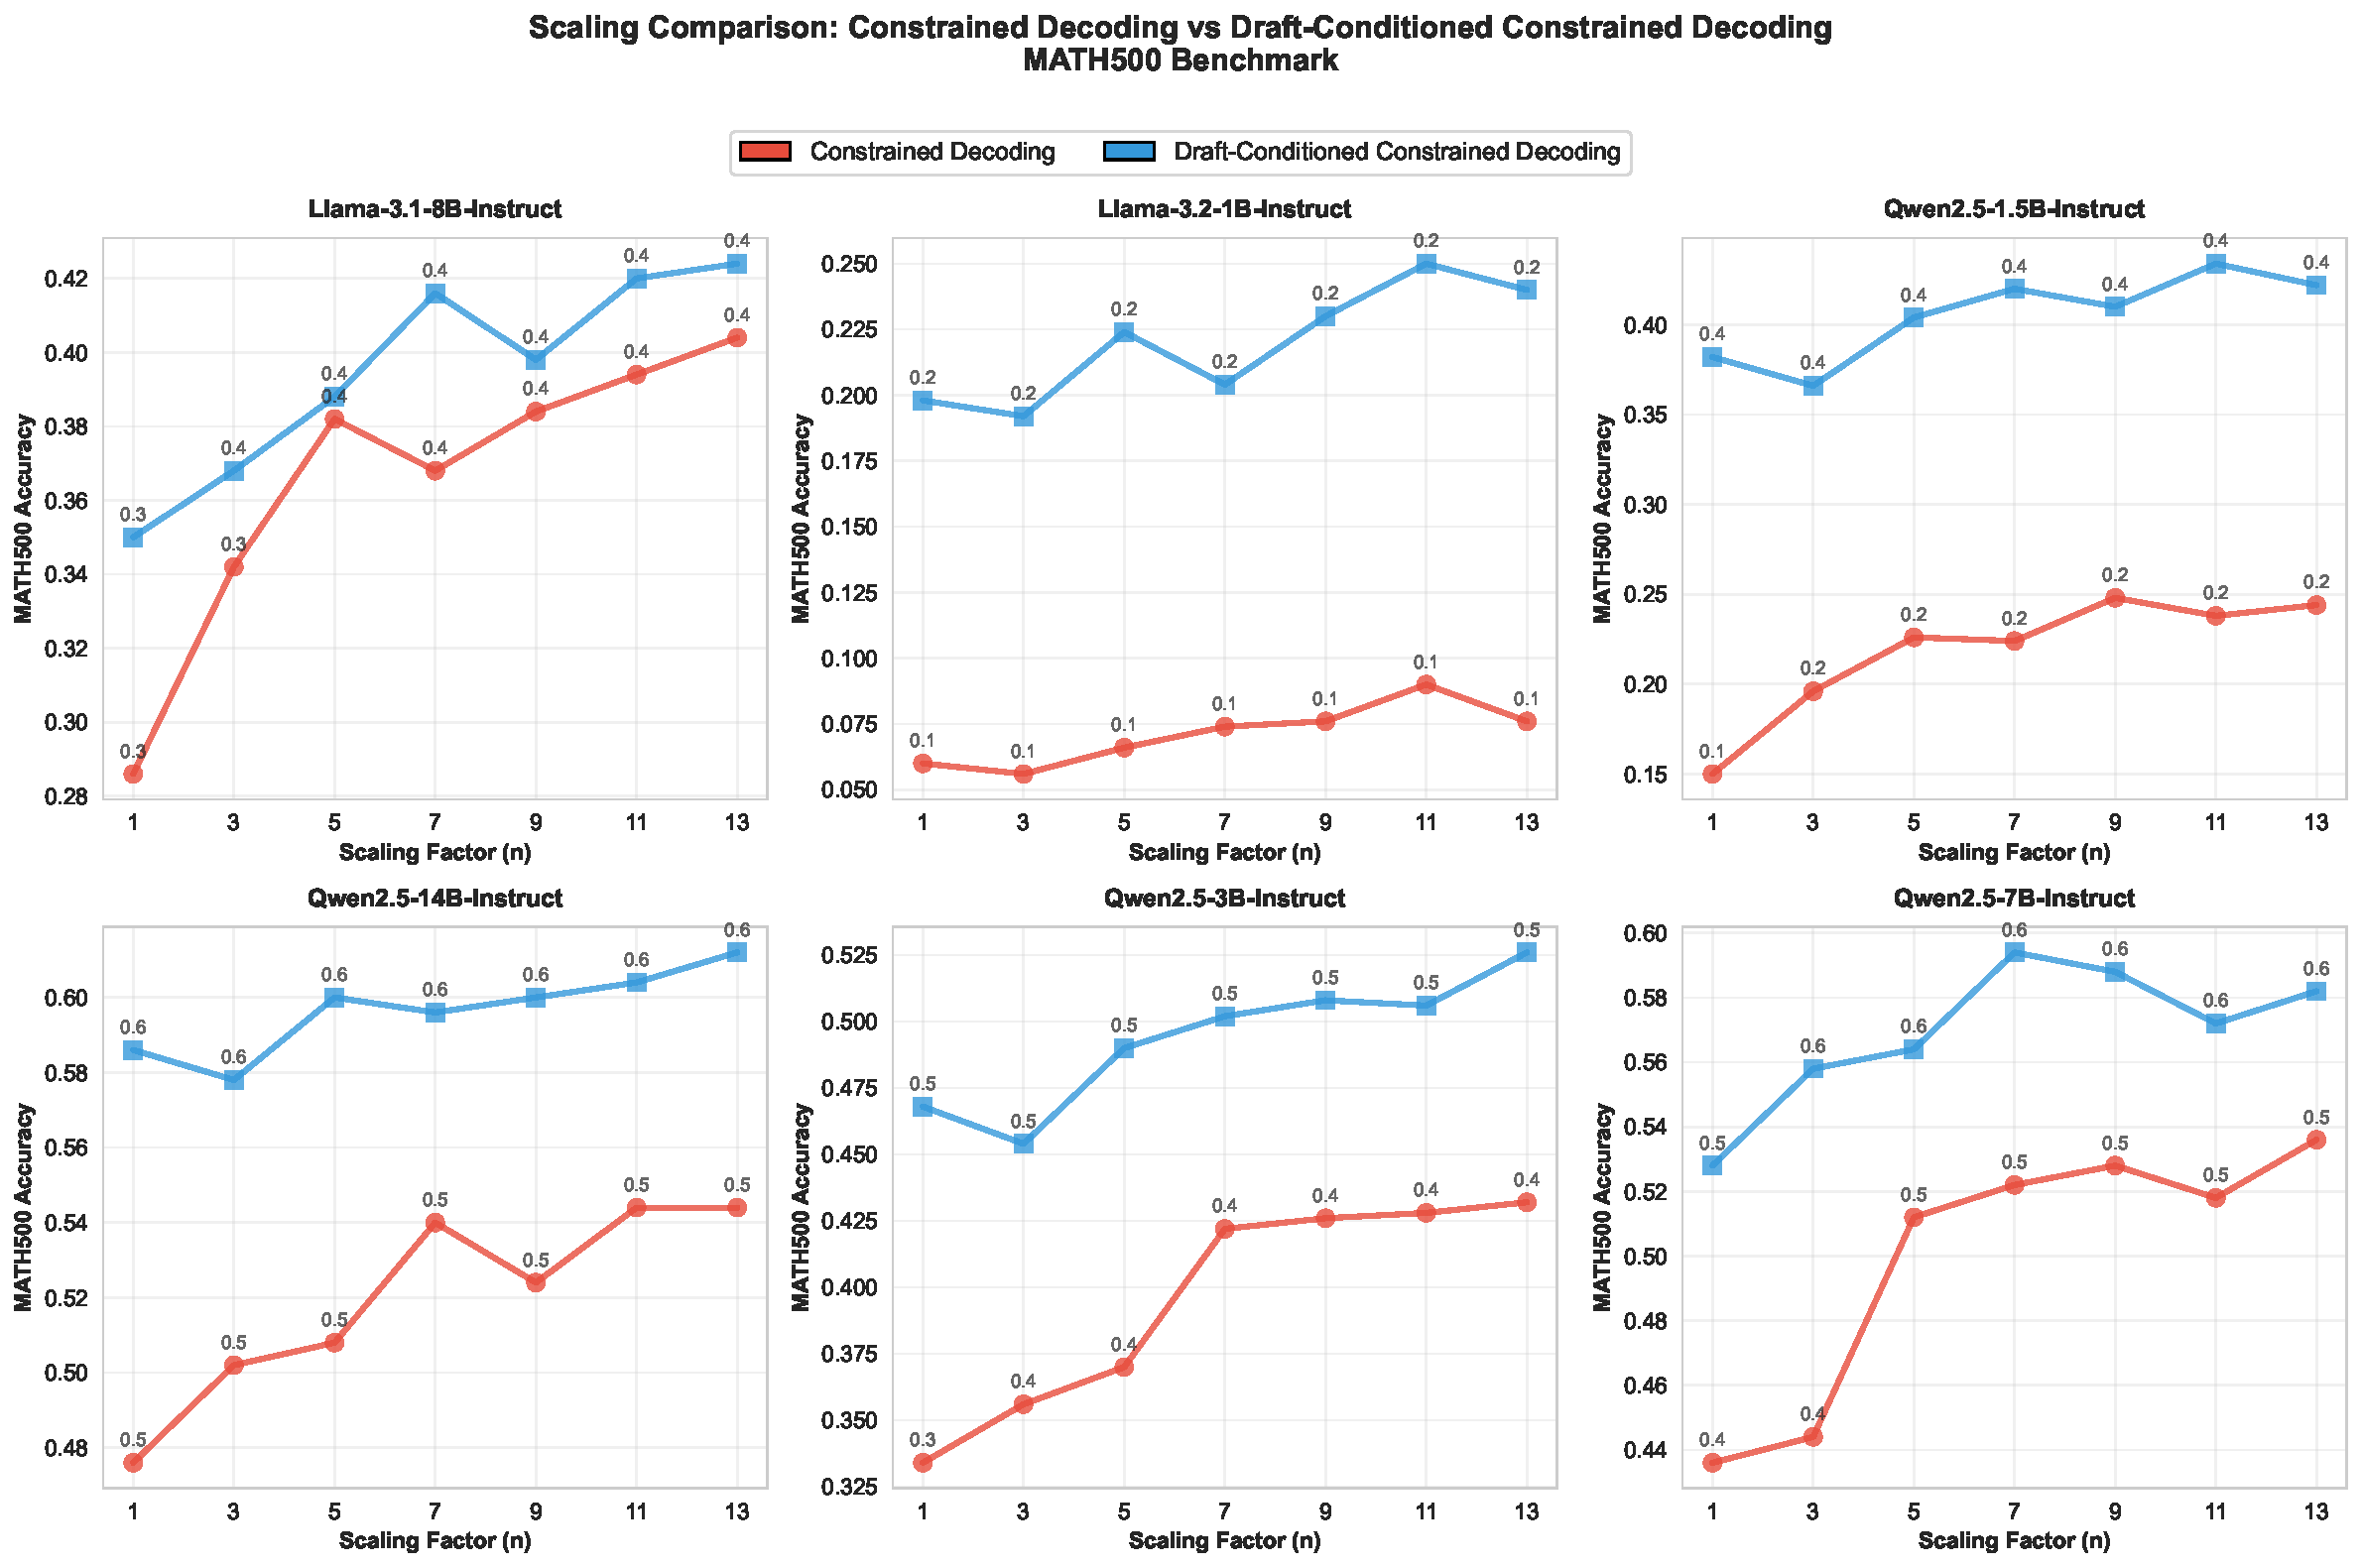
\includegraphics[width=0.9\linewidth]{figs/scaling_comparison_math500.pdf}
        \caption{MATH500 benchmark scaling results.}
        \label{fig:scaling_math500_detailed}
    \end{subfigure}
    
    \caption{Detailed test-time scaling comparison across all six models for GSM8K and MATH500 benchmarks. Each subplot shows the scaling behavior for a specific model, comparing Constrained Decoding(CD) (red) with Draft-Conditioned Constrained Decoding(DCCD) (blue). The consistent gap between methods across model sizes and benchmarks demonstrates the robustness of the DCCD approach.}
    \label{fig:scaling_detailed}
\end{figure*}


\section{Non-Verifiable Experimental Design and Evaluation}
\label{non-verifiable}
\subsection{Experimental Setup}

We conduct a non-verifiable evaluation comparing \textbf{Constrained Decoding (CD)} against \textbf{Draft Conditioned Constrained Decoding (DCCD)} across diverse prompt categories under a strict 256-token budget constraint. Without ground truth labels, we employ LLM-as-judge pairwise comparison to assess relative quality.

\paragraph{Constrained Decoding (CD)}
The model receives explicit instructions to generate content within a hard token budget ($\leq$256 tokens) while maintaining accuracy, coverage, and coherence. The prompt targets 95--100\% budget utilization with sentence-boundary termination.

\paragraph{Draft Conditioned Constrained Decoding (DCCD)}
Our proposed DCCD approach separates content generation from constraint satisfaction:

\begin{enumerate}
    \item \textbf{Draft Generation:} Generate a comprehensive, unconstrained answer focusing on accuracy, coverage, and reasoning. The model is informed of the downstream budget to ensure sufficient detail for compression.
    
    \item \textbf{Constrained Compression:} Compress the draft into a faithful summary within the hard budget, prioritizing coverage of core claims, key points, and critical numbers while avoiding fabrications.
\end{enumerate}

\textbf{Hypothesis:} Decoupling content generation from constraint satisfaction maintains reasoning quality while achieving structural constraints.

\begin{table}[h]
\centering
\caption{Evaluation prompt categories spanning diverse knowledge domains}
\label{tab:prompt_categories}
\begin{tabular}{@{}ll@{}}
\toprule
General Knowledge & Business \& Economics \\
Science \& Technology & AI \& Computer Science \\
Philosophy \& Psychology & Environment \& Sustainability \\
Culture, Media \& Design & Society, Law \& Policy \\
Health, Medicine \& Biology & Education \& Productivity \\
\bottomrule
\end{tabular}
\end{table}



\subsection{Evaluation Methodology}

\subsubsection{LLM-as-Judge Framework}

We employ \textbf{Qwen2.5-14B-Instruct} as an impartial evaluator for pairwise comparisons across three criteria: overall quality, coverage, and faithfulness. The judge produces structured XML output with explicit reasoning and a categorical decision (A/B/TIE).

\begin{tcolorbox}[colback=blue!5, colframe=blue!70!black, title=Judge System Prompt, fonttitle=\bfseries]
You are an impartial expert judge comparing two AI assistant answers. You MUST pick a single winner unless they are truly indistinguishable. Return XML with \texttt{<reasoning>...</reasoning>} and \texttt{<winner>A</winner>} or \texttt{<winner>B</winner>} or \texttt{<winner>TIE</winner>}. Do not include any other text outside the XML tags.
\end{tcolorbox}

\begin{tcolorbox}[colback=purple!5, colframe=purple!70!black, title=Judge User Prompt Template, fonttitle=\bfseries]
Compare two candidate answers to the same prompt. Decide which is BETTER under the given criterion, considering the hard constraint budget of \{budget\} tokens.

\textbf{PROMPT:} \{prompt\}

\textbf{CRITERION:} \{criterion\_explanation\}

\textbf{GENERAL RULES:}
\begin{itemize}
    \item Faithfulness: no invented facts; consistency with prompt
    \item Coverage: include essential points to satisfy the prompt
    \item Quality: clear, coherent, well-organized
    \item Constraint sensitivity: maintain essential information within budget
\end{itemize}

\textbf{CANDIDATE A:} \{answer\_a\} \quad \textbf{CANDIDATE B:} \{answer\_b\}

\textbf{OUTPUT:} \texttt{<reasoning>...</reasoning> <winner>A/B/TIE</winner>}
\end{tcolorbox}

\begin{tcolorbox}[colback=teal!5, colframe=teal!70!black, title=Evaluation Criteria, fonttitle=\bfseries]
\textbf{Overall Quality:} Prioritize correct, faithful, well-covered content that fits the budget and retains essential information.

\textbf{Coverage:} Prioritize answers that preserve essential points within budget while remaining clear and concise.

\textbf{Faithfulness:} Prioritize answers that avoid fabrications and remain faithful to the prompt while fitting the budget.
\end{tcolorbox}
\subsection{Results}

\begin{figure}[h!]
\centering
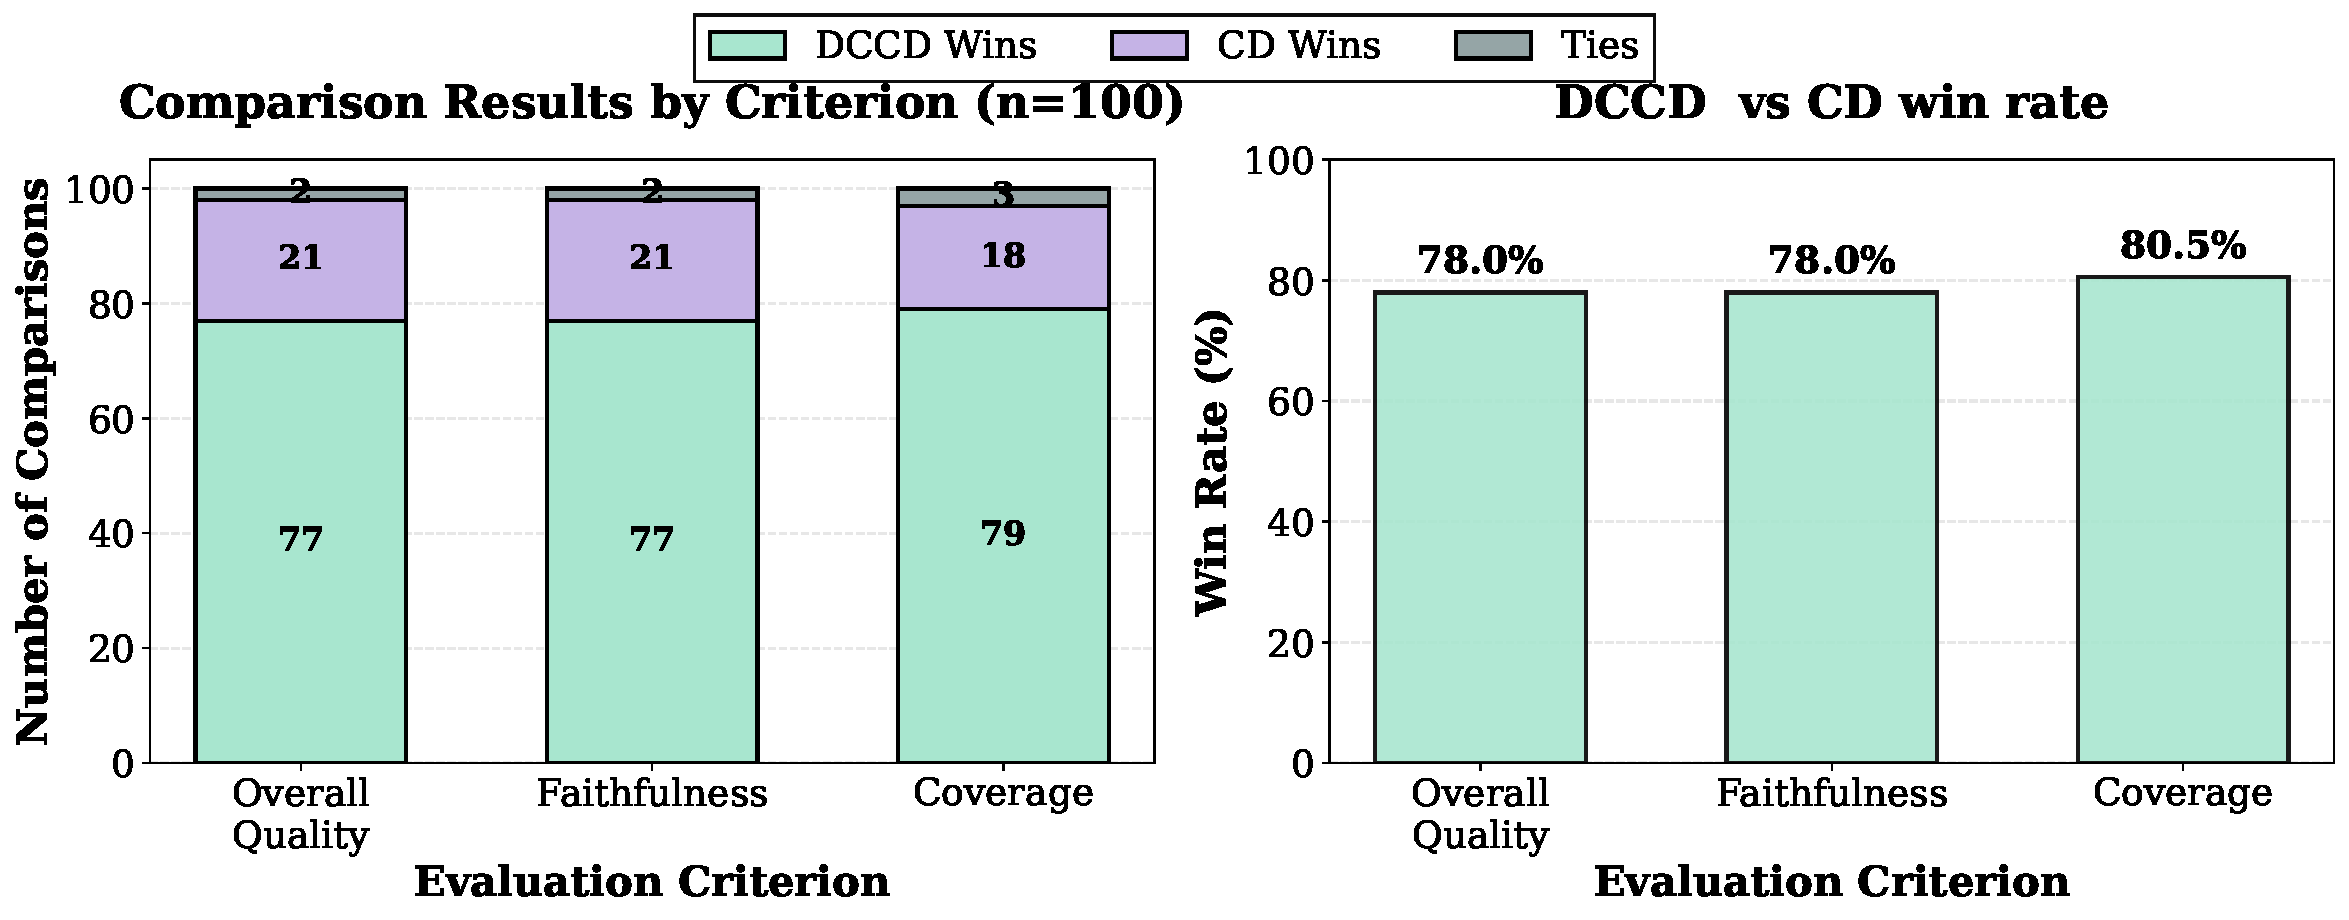
\includegraphics[width=\textwidth]{figs/dccd_vs_cd_results.pdf}
\caption{DCCD demonstrates consistent superiority across all evaluation criteria with win rates of 78--80.5\%. The highest performance on coverage (80.5\%) validates our hypothesis that separating reasoning from formatting preserves information density. The low tie rate (2--3\%) indicates clear quality differences, while robust performance across diverse prompt categories demonstrates generalizability. These findings confirm that explicit separation of content generation from constraint satisfaction maintains both reasoning quality and information completeness under hard token budgets.}
\label{fig:dccd_results}
\end{figure}



\section{Dataset Examples}
\label{app:dataset_examples}

This section provides complete examples from each benchmark dataset used in our evaluation, illustrating both the natural language questions and their corresponding structured outputs.

\subsection{GSM8K: Grade School Math}

\begin{tcolorbox}[
  enhanced,
  breakable,
  colback=green!5,
  colframe=green!50!black,
  boxrule=0.8pt,
  arc=2mm,
  left=5mm, right=5mm, top=3mm, bottom=3mm,
  fonttitle=\sffamily\bfseries,
  coltitle=black,
  attach boxed title to top left={xshift=3mm, yshift=-2mm},
  boxed title style={
    colback=green!10,
    colframe=green!50!black,
    boxrule=0.8pt,
    arc=1.5mm,
    left=2mm, right=2mm, top=1mm, bottom=1mm
  },
  before skip=6pt,
  after skip=10pt,
  title={GSM8K Example},
  width=\textwidth
]
\noindent\textbf{Question.}\\[3pt]
\emph{Janet's ducks lay 16 eggs per day. She eats three for breakfast every morning and bakes muffins for her friends every day with four. She sells the remainder at the farmers' market daily for \$2 per fresh duck egg. How much in dollars does she make every day at the farmers' market?}


\begin{figure*}[H]
\begin{tcolorbox}[ 
    enhanced,
  colback=gray!10,
  colframe=gray!80,
  boxrule=0.6pt,
  arc=2mm,
  left=2mm, right=2mm, top=1.2mm, bottom=1.2mm,
  fonttitle=\small\bfseries,
  coltitle=black,
  attach boxed title to top left={xshift=1.5mm, yshift=-1.5mm},
  boxed title style={
    colback=gray!10,
    colframe=black!40,
    boxrule=0.6pt,
    arc=1.5mm,
    left=1mm, right=1mm, top=0.6mm, bottom=0.6mm
  },
  before skip=4pt,
  after skip=6pt,
  title={Dataset Structural Constraints},
  width=\textwidth
]

\begin{minipage}[t]{0.32\textwidth}
\textbf{GSM8K \& MATH500}\\[2pt]
\textbf{Structural constraint:} JSON output with two fields:
\texttt{"steps"}: and \texttt{"answer"}.

\vspace{4pt}
\noindent\textbf{Expected structured output.}
\begin{lstlisting}[
  basicstyle=\ttfamily\scriptsize,
  breaklines=true,
  columns=fullflexible,
  keepspaces=true,
  showstringspaces=false,
  frame=none,
  xleftmargin=0pt,
  xrightmargin=0pt
]
{
  "steps": [
    "Description of Step 1",
    "Description of Step 2",
    "...",
    "Description of Step N"
  ],
  "answer": "Final Answer"
}
\end{lstlisting}
\end{minipage}%
\hfill
\begin{minipage}[t]{0.32\textwidth}
\textbf{GSM-Symbolic}\\[2pt]
\textbf{Structural constraint:}
Symbolic expression wrapped in Start delimter:   \texttt{<<} and ending delimiter \texttt{>>}, model must produce expression using the basic arithmetic operations only: \texttt{+}, \texttt{-}, \texttt{/}, \texttt{//}, \texttt{\%}, \texttt{()}, and \texttt{int()}.
\vspace{4pt}

\noindent\textbf{Expected structured output.}
\begin{lstlisting}[
  basicstyle=\ttfamily\scriptsize,
  breaklines=true,
  columns=fullflexible,
  keepspaces=true,
  showstringspaces=false,
  frame=none,
  xleftmargin=0pt,
  xrightmargin=0pt
]
<<symbolic_expression>>
\end{lstlisting}
\end{minipage}%
\hfill
\begin{minipage}[t]{0.32\textwidth}
\textbf{FOLIO}\\[2pt]
\textbf{Structural constraint:} Output containing three distinct components: {Predicates}, {Premises}, and {Conclusion}.
\vspace{1pt}
\noindent\textbf{Expected structured output.}
\begin{lstlisting}[
  basicstyle=\ttfamily\scriptsize,
  breaklines=true,
  columns=fullflexible,
  keepspaces=true,
  showstringspaces=false,
  frame=none,
  xleftmargin=0pt,
  xrightmargin=0pt
]
Predicates:
P(x) ::: description of P
Q(x) ::: description of Q
Premises:
forall x (P(x) implies Q(x))
  ::: premise description
Conclusion:
Q(a) ::: conclusion statement
\end{lstlisting}
\end{minipage}

\end{tcolorbox}
\caption{Structural constraints and expected outputs for each dataset used in our experiments.}
\label{fig:dataset_structures}
\end{figure*}

\vspace{6pt}
\noindent\textbf{Structured output.}
\begin{lstlisting}[
  basicstyle=\ttfamily\normalsize,
  breaklines=true,
  columns=fullflexible,
  keepspaces=true,
  showstringspaces=false,
  frame=none,
  xleftmargin=0pt,
  xrightmargin=0pt
]
{
  "steps": [
    "Calculate total eggs laid per day: 16",
    "Calculate eggs consumed daily: 3 + 4 = 7",
    "Calculate eggs remaining to sell: 16 - 7 = 9",
    "Calculate revenue at $2 per egg: 9 * 2 = 18"
  ],
  "answer": "18"
}
\end{lstlisting}
\end{tcolorbox}

\subsection{GSM-Symbolic: Symbolic Mathematical Reasoning}

\begin{tcolorbox}[
  enhanced,
  breakable,
  colback=green!5,
  colframe=green!50!black,
  boxrule=0.8pt,
  arc=2mm,
  left=5mm, right=5mm, top=3mm, bottom=3mm,
  fonttitle=\sffamily\bfseries,
  coltitle=black,
  attach boxed title to top left={xshift=3mm, yshift=-2mm},
  boxed title style={
    colback=green!10,
    colframe=green!50!black,
    boxrule=0.8pt,
    arc=1.5mm,
    left=2mm, right=2mm, top=1mm, bottom=1mm
  },
  before skip=6pt,
  after skip=10pt,
  title={GSM-Symbolic Example},
  width=\textwidth
]
\noindent\textbf{Question.}\\[3pt]
\emph{\{name\} makes \{drink\} using teaspoons of sugar and cups of water in the ratio of \{m\}:\{n\}. If she used a total of \{x\} teaspoons of sugar and cups of water, calculate the number of teaspoonfuls of sugar she used.}

\vspace{6pt}
\noindent\textbf{Structured output.}
\begin{lstlisting}[
  basicstyle=\ttfamily\normalsize,
  breaklines=true,
  columns=fullflexible,
  keepspaces=true,
  showstringspaces=false,
  frame=none,
  xleftmargin=0pt,
  xrightmargin=0pt
]
{
  "answer": "<<(m*x)//(m+n)>>"
}
\end{lstlisting}
\end{tcolorbox}

\subsection{FOLIO: First-Order Logic Reasoning}

\begin{tcolorbox}[
  enhanced,
  breakable,
  colback=green!5,
  colframe=green!50!black,
  boxrule=0.8pt,
  arc=2mm,
  left=5mm, right=5mm, top=3mm, bottom=3mm,
  fonttitle=\sffamily\bfseries,
  coltitle=black,
  attach boxed title to top left={xshift=3mm, yshift=-2mm},
  boxed title style={
    colback=green!10,
    colframe=green!50!black,
    boxrule=0.8pt,
    arc=1.5mm,
    left=2mm, right=2mm, top=1mm, bottom=1mm
  },
  before skip=6pt,
  after skip=10pt,
  title={FOLIO Example},
  width=\textwidth
]
\noindent\textbf{Question.}\\[3pt]
\emph{All people who regularly drink coffee are dependent on caffeine. People either regularly drink coffee or joke about being addicted to caffeine. No one who jokes about being addicted to caffeine is unaware that caffeine is a drug. Rina is either a student and unaware that caffeine is a drug, or neither a student nor unaware that caffeine is a drug.}

\vspace{3pt}
\emph{Is the following statement true, false, or uncertain? Rina is either a person who jokes about being addicted to caffeine or is unaware that caffeine is a drug.}

\vspace{6pt}
\noindent\textbf{Structured output.}
\begin{lstlisting}[
  basicstyle=\ttfamily\normalsize,
  breaklines=true,
  columns=fullflexible,
  keepspaces=true,
  showstringspaces=false,
  frame=none,
  xleftmargin=0pt,
  xrightmargin=0pt
]
Predicates:
Dependent(x) ::: x is dependent on caffeine
Drinks(x) ::: x regularly drinks coffee
Jokes(x) ::: x jokes about being addicted to caffeine
Unaware(x) ::: x is unaware that caffeine is a drug
Student(x) ::: x is a student

Premises:
forall x (Drinks(x) implies Dependent(x)) ::: All coffee drinkers are dependent on caffeine
forall x (Drinks(x) xor Jokes(x)) ::: People either drink coffee or joke about caffeine addiction
forall x (Jokes(x) implies not Unaware(x)) ::: Those who joke are aware caffeine is a drug
(Student(rina) and Unaware(rina)) xor not (Student(rina) or Unaware(rina)) ::: Rina's student and awareness status

Conclusion:
Jokes(rina) xor Unaware(rina) ::: Rina jokes about caffeine or is unaware it is a drug
\end{lstlisting}
\end{tcolorbox}


\section{Few-Shot Examples for Constrained Few-Shot Baseline}
\label{app:few_shot_examples}

This section presents the in-context examples used in the Constrained Few-Shot baseline for each dataset.

\subsection{GSM8K Few-Shot Examples}

\begin{tcolorbox}[colback=gray!10, colframe=black]
\textbf{Example 1}
\begin{verbatim}
{
  "steps": [
    "Natalia sold 48 clips in April.",
    "She sold half as many clips in May, which is 24.",
    "Adding April and May sales gives 48 + 24."
  ],
  "answer": "72"
}
\end{verbatim}

\tcblower

\textbf{Example 2}
\begin{verbatim}
{
  "steps": [
    "Babysitting rate is 12 dollars per hour.",
    "50 minutes equals 5/6 of an hour.",
    "Multiply 12 by 5/6 to get earnings."
  ],
  "answer": "10"
}
\end{verbatim}

\tcblower

\textbf{Example 3}
\begin{verbatim}
{
  "steps": [
    "The wallet costs 100 dollars.",
    "Betty has half the money, which is 50.",
    "Her parents give 15 dollars and her grandparents give 30 dollars.",
    "Total money becomes 95, so subtract from 100."
  ],
  "answer": "5"
}
\end{verbatim}

\tcblower

\textbf{Example 2}
\begin{verbatim}
{
  "steps": [
    "The book has 120 pages total.",
    "Julie read 12 pages yesterday and 24 pages today.",
    "She has read 36 pages, leaving 84 pages.",
    "Half of the remaining pages is 42."
  ],
  "answer": "42"
}
\end{verbatim}
\end{tcolorbox}

\subsection{MATH500 Few-Shot Examples}

\begin{tcolorbox}[colback=gray!10, colframe=black]
\textbf{Example 1}
\begin{verbatim}
{
  "steps": [
    "Continuity at $x=2$ requires $a(2)+3 = 2-5$.",
    "Solving gives $2a+3=-3$ so $a=-3$.",
    "Continuity at $x=-2$ requires $2(-2)-b = -2-5$.",
    "Solving gives $-4-b=-7$ so $b=3$.",
    "Thus $a+b=-3+3$."
  ],
  "answer": "0"
}
\end{verbatim}

\tcblower

\textbf{Example 2}
\begin{verbatim}
{
  "steps": [
    "Let the original formation have $m$ members per row and $r$ rows, 
     so the total is $mr+2$.",
    "The new formation has $(m+1)$ members per row and $(r-2)$ rows, 
     so $(m+1)(r-2)=mr+2$.",
    "Expanding gives $mr-2m+r-2=mr+2$ which simplifies to $r=2m+4$.",
    "Total members are $N=mr+2=m(2m+4)+2=2m^2+4m+2$.",
    "Impose $N<100$ and choose the largest valid integer.",
    "This yields $N=98$."
  ],
  "answer": "98"
}
\end{verbatim}

\tcblower

\textbf{Example 3}
\begin{verbatim}
{
  "steps": [
    "Combine constant terms $4+100+9$ into a single constant.",
    "Identify the highest power of $x$ in the polynomial.",
    "The highest-degree terms are $2\pi x^4$ and $\sqrt{10}x^4$.",
    "Therefore the degree of the polynomial is $4$."
  ],
  "answer": "4"
}
\end{verbatim}

\tcblower

\textbf{Example 2}
\begin{verbatim}
{
  "steps": [
    "Let $w$ be the number of days Sam worked.",
    "He did not work $20-w$ days.",
    "Total earnings are $60w-30(20-w)=660$.",
    "Solving gives $90w=1260$ so $w=14$.",
    "Days not worked are $20-14$."
  ],
  "answer": "6"
}
\end{verbatim}
\end{tcolorbox}

\subsection{GSM-Symbolic Few-Shot Examples}

\begin{tcolorbox}[colback=gray!10, colframe=black]
\begin{verbatim}
<<tf - t>>
<<c + nc>>
<<ch1 + ch2 - a>>
<<l1 - g>>
<<t + tm + td>>
<<c + nc * (d2 - d1 + 1)>>
<<gb1 - l1 - l2>>
<<m - q * p>>
\end{verbatim}
\end{tcolorbox}

\subsection{FOLIO Few-Shot Examples}

\begin{tcolorbox}[colback=gray!10, colframe=black]
\textbf{Example 1: Coffee and Caffeine}
\begin{verbatim}
Predicates:
Dependent(x) ::: x is a person dependent on caffeine.
Drinks(x) ::: x regularly drinks coffee.
Jokes(x) ::: x jokes about being addicted to caffeine.
Unaware(x) ::: x is unaware that caffeine is a drug.
Student(x) ::: x is a student.

Premises:
forall x (Drinks(x) implies Dependent(x)) ::: All people who regularly 
  drink coffee are dependent on caffeine.
forall x (Drinks(x) xor Jokes(x)) ::: People either regularly drink 
  coffee or joke about being addicted to caffeine.
forall x (Jokes(x) implies not Unaware(x)) ::: No one who jokes about 
  being addicted to caffeine is unaware that caffeine is a drug.
(Student(rina) and Unaware(rina)) xor not (Student(rina) or Unaware(rina)) 
  ::: Rina is either a student and unaware that caffeine is a drug, or 
  neither a student nor unaware that caffeine is a drug.

Conclusion:
Jokes(rina) xor Unaware(rina) ::: Rina is either a person who jokes about 
  being addicted to caffeine or is unaware that caffeine is a drug.
\end{verbatim}

\tcblower

\textbf{Example 2: Choral Conductor}
\begin{verbatim}
Predicates:
Czech(x) ::: x is a Czech person.
ChoralConductor(x) ::: x is a choral conductor.
Musician(x) ::: x is a musician.
Love(x, y) ::: x loves y.
Author(x, y) ::: x is the author of y.
Book(x) ::: x is a book.
Publish(x, y) ::: x is published in year y.
Specialize(x, y) ::: x specializes in y.

Premises:
Czech(miroslav) and ChoralConductor(miroslav) and 
  Specialize(miroslav, renaissance) and Specialize(miroslav, baroque) 
  ::: Miroslav Venhoda was a Czech choral conductor who specialized in 
  the performance of Renaissance and Baroque music.
forall x (ChoralConductor(x) implies Musician(x)) ::: Any choral 
  conductor is a musician.
exists x (Musician(x) and Love(x, music)) ::: Some musicians love music.
Book(methodOfStudyingGregorianChant) and 
  Author(miroslav, methodOfStudyingGregorianChant) and 
  Publish(methodOfStudyingGregorianChant, year1946) ::: Miroslav Venhoda 
  published a book in 1946 called Method of Studying Gregorian Chant.

Conclusion:
Love(miroslav, music) ::: Miroslav Venhoda loved music.
\end{verbatim}

\tcblower

\textbf{Example 3: Whales and Mammals}
\begin{verbatim}
Predicates:
Mammal(x) ::: x is a mammal.
Whale(x) ::: x is a whale.
Fish(x) ::: x is a fish.
LivesInWater(x) ::: x lives in water.

Premises:
forall x (Whale(x) implies Mammal(x)) ::: All whales are mammals.
forall x (Whale(x) implies LivesInWater(x)) ::: All whales live in water.
Whale(willy) ::: Willy is a whale.
forall x (Fish(x) implies LivesInWater(x)) ::: All fish live in water.
forall x (Mammal(x) implies not Fish(x)) ::: No mammal is a fish.

Conclusion:
not Fish(willy) ::: Willy is not a fish.
\end{verbatim}

\tcblower

\textbf{Example 2: Even and Odd Integers}
\begin{verbatim}
Predicates:
Even(x) ::: x is even.
Odd(x) ::: x is odd.
Integer(x) ::: x is an integer.
Sum(x, y, z) ::: z is the sum of x and y.

Premises:
Integer(a) and Integer(b) ::: a and b are integers.
Even(a) ::: a is even.
Odd(b) ::: b is odd.
forall x (forall y ((Even(x) and Odd(y)) implies Odd(x+y))) ::: The sum 
  of an even integer and an odd integer is odd.

Conclusion:
Odd(a+b) ::: a+b is odd.
\end{verbatim}
\end{tcolorbox}


\section{System Prompts for Constrained Prompting Baseline}
\label{app:constrained_prompts}

This section presents the carefully engineered system prompts used in the Constrained Prompting baseline for each dataset. These prompts specify the required output structure and format constraints.



\subsection{GSM8K and MATH500 System Prompt}

\begin{tcolorbox}[colback=gray!10, colframe=black]
\begin{verbatim}
You are a meticulous math tutor. Solve the problem step by step and 
OUTPUT ONLY a single JSON object conforming to the provided schema, 
'{steps: string[], answer: string}'. No extra text, no code fences, 
no commentary outside JSON.

{
  "steps": [
    "Step 1",
    "Step 2",
    "...",
    "Step N"
  ],
  "answer": "Final Answer"
}

Result in 'answer'. No extra text, no code fences, no commentary 
outside JSON.
\end{verbatim}
\end{tcolorbox}

\subsection{GSM-Symbolic System Prompt}

\begin{tcolorbox}[colback=gray!10, colframe=black]
\begin{verbatim}
Only output the symbolic expression wrapped in [[START]] [[END]] that 
answers the question. The expression must use numbers as well as the 
variables defined in the question. You are only allowed to use the 
following operations: +, -, /, //, %, (), and int().

You will always respond in the format described below: 
[[START]]symbolic expression[[END]]
\end{verbatim}
\end{tcolorbox}

\subsection{FOLIO System Prompt}

\begin{tcolorbox}[colback=gray!10, colframe=black]
\begin{verbatim}
Given a problem description and a question. The task is to parse the 
problem and the question into first-order logic formulas.

The grammar of the first-order logic formula is defined as follows:
1) logical conjunction of expr1 and expr2: expr1 {and} expr2
2) logical disjunction of expr1 and expr2: expr1 {or} expr2
3) logical exclusive disjunction of expr1 and expr2: expr1 {xor} expr2
4) logical negation of expr1: {not}expr1
5) expr1 implies expr2: expr1 {implies} expr2
6) expr1 if and only if expr2: expr1 {iff} expr2
7) logical universal quantification: {forall} x
8) logical existential quantification: {exists} x

These are the ONLY operations in the grammar.

Expected output format:
Predicates:
P(x) ::: description of P
Q(x) ::: description of Q

Premises:
forall x (P(x) implies Q(x)) ::: premise description

Conclusion:
Q(a) ::: conclusion statement

------
Given the message above, Just write the "Predicates:", "Premises:", 
and "Conclusion:" fields. DO NOT OUTPUT ANYTHING ELSE OTHER THAN THE 
ANSWER! Answer the question EXACTLY like the examples.
\end{verbatim}
\end{tcolorbox}

\section{Constraints for Constrained Decoding Baseline}
\label{app:constrained_decoding}

This section presents the formal constraints used in the Constrained Decoding baseline with XGrammar. For JSON-based tasks, we use Pydantic schemas, while symbolic and logical tasks use context-free grammars.

\subsection{GSM8K Schema}

\begin{tcolorbox}[colback=gray!10, colframe=black]
\begin{verbatim}
class GSM8KSchema(BaseModel):
    steps: Annotated[List[str], Field(min_length=1)]
    answer: Annotated[str, Field(min_length=1)]
\end{verbatim}
\end{tcolorbox}

\subsection{MATH500 Schema}

\begin{tcolorbox}[colback=gray!10, colframe=black]
\begin{verbatim}
class MATHSchema(BaseModel):
    steps: Annotated[List[str], Field(min_length=1)]
    answer: Annotated[str, Field(min_length=1)]
\end{verbatim}
\end{tcolorbox}

\subsection{GSM-Symbolic Grammar}

\begin{tcolorbox}[colback=gray!10, colframe=black]
\begin{verbatim}
start: space? "<" "<" space? expr space? ">" ">" space?

expr: expr space? "+" space? term   
     | expr space? "-" space? term   
     | term

term: term space? "*" space? factor 
     | term space? "/" space? factor 
     | term space? "//" space? factor 
     | term space? "%" space? factor  
     | factor space?

factor: "-" space? factor    
       | TYPE "(" space? expr space? ")" 
       | primary space?

primary: NUMBER        
        | VARIABLE      
        | "(" space? expr space? ")"

TYPE: "int"

space: " "

%import common.CNAME -> VARIABLE
%import common.NUMBER
\end{verbatim}
\end{tcolorbox}

\subsection{FOLIO Grammar}



\begin{tcolorbox}[colback=gray!10, colframe=black]
\small
\begin{lstlisting}[
  basicstyle=\ttfamily\small,
  breaklines=true,
  columns=fullflexible,
  keepspaces=true,
  showstringspaces=false,
  frame=none,
  escapechar=@
]
start: predicate_section premise_section conclusion_section

predicate_section: "Predicates:" predicate_definition+
premise_section: "Premises:" premise+
conclusion_section: "Conclusion:" conclusion+

predicate_definition: PREDICATE "(" VAR ("," VAR)* ")" COMMENT  
                      -> define_predicate
premise: quantified_expr COMMENT -> define_premise
conclusion: quantified_expr COMMENT -> define_conclusion

quantified_expr: quantifier VAR "(" expression ")" | expression
quantifier: "@$\forall$@" -> forall | "@$\exists$@" -> exists

expression: bimplication_expr

?bimplication_expr: implication_expr ("@$\leftrightarrow$@" bimplication_expr)?  -> iff
?implication_expr: xor_expr ("@$\rightarrow$@" implication_expr)?  -> imply
?xor_expr: or_expr ("@$\oplus$@" xor_expr)?  -> xor
?or_expr: and_expr ("@$\vee$@" or_expr)?  -> or
?and_expr: neg_expr ("@$\wedge$@" and_expr)?  -> and
?neg_expr: "@$\neg$@" quantified_expr  -> neg 
        | atom

?atom: PREDICATE "(" VAR ("," VAR)* ")" -> predicate 
    | "(" quantified_expr ")" 

// Variable names begin with a lowercase letter
VAR: /[a-z][a-zA-Z0-9_]*/  | /[0-9]+/

// Predicate names begin with a capital letter
PREDICATE: /[A-Z][a-zA-Z0-9]*/

COMMENT: /:::.*\n/

%import common.WS
%ignore WS
\end{lstlisting}
\end{tcolorbox}


\section{Case Study: Why Draft-Conditioned Constrained Decoding Works}
\label{app:case_study}

This section presents a detailed example demonstrating why Draft-Conditioned Constrained Decoding outperforms other approaches. We show how constrained decoding can harm reasoning quality, while our DCCD approach preserves both correctness and structure.

\subsection{Problem Statement}

\begin{tcolorbox}[colback=blue!5, colframe=blue!40, title={MATH500 Problem}]
Define
\[p = \sum_{k = 1}^\infty \frac{1}{k^2} \quad \text{and} \quad q = \sum_{k = 1}^\infty \frac{1}{k^3}.\]
Find a way to write
\[\sum_{j = 1}^\infty \sum_{k = 1}^\infty \frac{1}{(j + k)^3}\]
in terms of $p$ and $q$.\\
\noindent\textbf{Ground Truth Answer:} $\boxed{p - q}$
\end{tcolorbox}


\subsection{Baseline Predictions}

\subsubsection{Constrained Decoding (XGrammar) - INCORRECT}

\begin{tcolorbox}[colback=red!5, colframe=red!60!black]
\begin{lstlisting}[
  basicstyle=\ttfamily\small,
  breaklines=true,
  columns=fullflexible,
  keepspaces=true,
  showstringspaces=false,
  frame=none
]
{
  "steps": [
    "Given the sums p and q, we start by examining the double sum ...",
    "We can change the order of summation. Let's denote m = j + k. For each m, j can range from 1 to m - 1.",
    "Thus, we can rewrite the double sum as ...",
    "Now, let's expand the inner sum. We need to find ...",
    "The inner sum is a constant 1/m3 summed m-1 times, thus it equals (m-1) / m3.",
    "So, the expression becomes ...",
    "We can split the fraction ...",
    "This can be written as ...",
    "We know that the sum of 1/m3 is q and the sum of 1/m4 is a term related to the Riemann zeta function (4) = p^2/3.",
    "Therefore, the expression becomes q - p^2/3.",
    "The final answer is q - p^2/3."
  ],
  "answer": "q - p^2/3"
}
\end{lstlisting}
\tcblower
\noindent\textbf{Analysis:} The model produces valid JSON but makes a critical mathematical error: it incorrectly claims that $\sum_{m=2}^\infty \frac{1}{m^4} = \frac{p^2}{3}$, leading to the wrong answer $q - \frac{p^2}{3}$.
\end{tcolorbox}


\subsubsection{Constrained Prompting - INCOMPLETE/MALFORMED}

\begin{tcolorbox}[colback=red!5, colframe=red!60!black]
\begin{lstlisting}[
  basicstyle=\ttfamily\small,
  breaklines=true,
  columns=fullflexible,
  keepspaces=true,
  showstringspaces=false,
  frame=none
]
{
  "steps": [
    "Express the double sum as a sum over all pairs (j, k) where j and k are positive integers.",
    "Notice that each term 1/(j+k)^3 appears in the sum when j and k are such that j + k = n, for n ranging from 2 to infinity.",
    "For each n, the term 1/n^3 appears in the sum for all pairs (j, k) such that j + k = n, specifically for j = 1 to n-1.",
    "Thus, we can write the double sum as a sum over n from 2 to infinity, where the contribution for each n is 1/n^3 times the number of pairs (j, k) such that j + k = n.",
    "The number of such pairs is n-1, giving us sum_{n=2}^infty (n-1)/n^3.",
    "Rewrite the sum as sum_{n=2}^infty (n-1)/n^3 = sum_{n=2}^infty (1/n^2 - 1/n^3)",
    "Separate the sums: sum_{n=2}^infty 1/n^2 - sum_{n=2}^infty 1/n^3.",
    "Recognize that sum_{n=2}^infty 1/n^2 = p - 1 and sum_{n=2}^infty 1/n^3 = q - 1.",
    "Therefore, the final expression is (p - 1) - (q
\end{lstlisting}
\tcblower
\noindent\textbf{Analysis:} The reasoning is mathematically correct and would lead to the right answer $(p-1)-(q-1) = p-q$, but the output is truncated mid-sentence and produces invalid JSON. The structure constraint is violated.
\end{tcolorbox}


\subsubsection{Constrained Few-Shot - INCOMPLETE/MALFORMED}

\begin{tcolorbox}[colback=red!5, colframe=red!60!black]
\begin{lstlisting}[
  basicstyle=\ttfamily\small,
  breaklines=true,
  columns=fullflexible,
  keepspaces=true,
  showstringspaces=false,
  frame=none
]
{
  "steps": [
    "First, consider the double sum $\sum_{j=1}^\infty \sum_{k=1}^\infty \frac{1}{(j+k)^3}$. We can change the order of summation to make the expression more manageable.",
    "Let $n = j + k$. Then, for a fixed $n$, $j$ ranges from $1$ to $n-1$ and $k = n - j$. Therefore, the double sum can be rewritten as $\sum_{n=2}^\infty \sum_{j=1}^{n-1} \frac{1}{n^3}$.",
    "The inner sum is $\sum_{j=1}^{n-1} \frac{1}{n^3} = \frac{n-1}{n^3} = \frac{1}{n^2} - \frac{1}{n^3}$. Thus the double sum becomes $\sum_{n=2}^\infty \left( \frac{1}{n^2} - \frac{1}{n^3} \right)$.",
    "This can be split into two separate sums: $\sum_{n=2}^\infty \frac{1}{n^2} - \sum_{n=2}^\infty \frac{1}{n^3}$.",
    "Recognize that $\sum_{n=2}^\infty \frac{1}{n^2} = \sum_{n=1}^\infty \frac{1}{n^2} - \frac{1}{1^2} = p - 1$ and $\sum_{n=2}^\infty \frac{1}{n^3} = \sum_{n=1}^\infty \frac{1}{n^3} - \frac{1}{
\end{lstlisting}
\tcblower
\noindent\textbf{Analysis:} Despite providing few-shot examples, the model output is truncated mid-expression within the last step. The reasoning up to the truncation point is mathematically correct and would lead to the answer $(p-1)-(q-1) = p-q$, but the output produces \textcolor{red}{invalid JSON} due to incomplete string and missing closing brackets. Both the answer field and proper JSON structure are absent.
\end{tcolorbox}


\subsection{Draft-Conditioned Constrained Decoding}

\subsubsection{Stage 1: Unconstrained Reasoning Generation}

\begin{tcolorbox}[colback=blue!5, colframe=blue!40, title={Stage 1 Output}]
\small
To find a way to express $\displaystyle\sum_{j = 1}^\infty \sum_{k = 1}^\infty \frac{1}{(j + k)^3}$ in terms of $p$ and $q$, we need to carefully analyze and manipulate the given double sum. Let's start by examining the structure of the sum.

First, let's rewrite the double sum in a more convenient form:
\[
\sum_{j = 1}^\infty \sum_{k = 1}^\infty \frac{1}{(j + k)^3}.
\]

We can change the order of summation. To do this, we need to consider the range of $j + k$. For a fixed $n = j + k$, $j$ can range from 1 to $n-1$ and $k$ can range from 1 to $n-1$. Therefore, we can rewrite the sum as:
\[
\sum_{n = 2}^\infty \sum_{j = 1}^{n-1} \frac{1}{n^3}.
\]

Now, let's simplify the inner sum:
\[
\sum_{j = 1}^{n-1} \frac{1}{n^3} = \frac{1}{n^3} \sum_{j = 1}^{n-1} 1 = \frac{1}{n^3} (n-1) = \frac{n-1}{n^3}.
\]

Substituting this back into the outer sum, we get:
\[
\sum_{n = 2}^\infty \frac{n-1}{n^3}.
\]

We can split the fraction:
\[
\sum_{n = 2}^\infty \frac{n-1}{n^3} = \sum_{n = 2}^\infty \left( \frac{n}{n^3} - \frac{1}{n^3} \right) = \sum_{n = 2}^\infty \frac{1}{n^2} - \sum_{n = 2}^\infty \frac{1}{n^3}.
\]

We can separate the sums:
\[
\sum_{n = 2}^\infty \frac{1}{n^2} = \left( \sum_{n = 1}^\infty \frac{1}{n^2} \right) - 1 = p - 1,
\]
\[
\sum_{n = 2}^\infty \frac{1}{n^3} = \left( \sum_{n = 1}^\infty \frac{1}{n^3} \right) - 1 = q - 1.
\]

Substituting these results back into our expression, we get:
\[
\sum_{n = 2}^\infty \frac{n-1}{n^3} = (p - 1) - (q - 1) = p - q.
\]

Thus, the final answer is:
\[
\boxed{p - q}.
\]
\end{tcolorbox}

\subsubsection{Stage 2: Structure Conversion}

\begin{tcolorbox}[colback=green!5, colframe=green!50!black, title={Stage 2 Output}]
\begin{lstlisting}[
  basicstyle=\ttfamily\small,
  breaklines=true,
  columns=fullflexible,
  keepspaces=true,
  showstringspaces=false,
  frame=none
]
{
  "steps": [
    "Rewrite the double sum $\sum_{j=1}^\infty \sum_{k=1}^\infty \frac{1}{(j+k)^3}$ in a more convenient form",
    "Change the order of summation: for fixed $n = j + k$, rewrite as $\sum_{n=2}^\infty \sum_{j=1}^{n-1} \frac{1}{n^3}$",
    "Simplify the inner sum: $\sum_{j=1}^{n-1} \frac{1}{n^3} = \frac{n-1}{n^3}$",
    "Substitute back into the outer sum to get $\sum_{n=2}^\infty \frac{n-1}{n^3}$",
    "Split the fraction: $\sum_{n=2}^\infty \frac{n-1}{n^3} = \sum_{n=2}^\infty \frac{1}{n^2} - \sum_{n=2}^\infty \frac{1}{n^3}$",
    "Separate the sums: $\sum_{n=2}^\infty \frac{1}{n^2} = p - 1$ and $\sum_{n=2}^\infty \frac{1}{n^3} = q - 1$",
    "Substitute the results: $(p - 1) - (q - 1) = p - q$"
  ],
  "answer": "p - q"
}
\end{lstlisting}
\tcblower
\noindent\textbf{Analysis:} Stage 2 successfully converts the unconstrained reasoning from Stage 1 into perfectly valid JSON structure. The model extracts the key reasoning steps, preserves mathematical notation, and produces both the correct answer $p - q$ (\textcolor{green!50!black}{CORRECT}) and valid JSON structure (\textcolor{green!50!black}{VALID}). This demonstrates how Draft-Conditioned Constrained Decoding achieves both goals: high-quality reasoning from Stage 1 and strict format compliance from Stage 2.
\end{tcolorbox}



\section{Additional Case Study: GSM-Symbolic}
\label{app:gsm_symbolic_case}
\begin{tcolorbox}[colback=blue!5, colframe=blue!40, title={GSM-Symbolic Problem}]
\texttt{\{name\}} was preparing for a \texttt{\{event\}} at her house, where she intended to serve \texttt{\{food\}}. She noticed that she was out of plastic \texttt{\{obj\}}, so she bought a new package of \texttt{\{obj\}}. Later, her husband also bought a package of \texttt{\{n1\}} new \texttt{\{obj\}} and gave them to \texttt{\{name\}}. While \texttt{\{name\}} was making the \texttt{\{food\}}, she used \texttt{\{n2\}} of the \texttt{\{obj\}} to sample her \texttt{\{food\}}. Later, when she went to set the table, she had a total of \texttt{\{total\}} \texttt{\{obj\}}. How many \texttt{\{obj\}} were in the package that \texttt{\{name\}} bought?

\vspace{3pt}
\noindent\textbf{Ground Truth:} \texttt{total + n2 - n1}
\begin{tcolorbox}[colback=gray!10, colframe=black, title={Baseline Predictions}]
\textbf{Constrained Decoding (XGrammar): \textcolor{red}{INCORRECT}}
\begin{lstlisting}[aboveskip=2pt, belowskip=2pt]
<<total - n2 + n1>>
\end{lstlisting}
\vspace{-2pt}
\noindent\rule{\textwidth}{0.4pt}

\textbf{Constrained Prompting: \textcolor{red}{INCORRECT} }
\begin{lstlisting}[aboveskip=2pt, belowskip=2pt]
<<total - n2 - n1>>
\end{lstlisting}
\vspace{-2pt}
\noindent\rule{\textwidth}{0.4pt}

\textbf{Constrained Few-Shot: \textcolor{red}{INCORRECT}}
\begin{lstlisting}[aboveskip=2pt, belowskip=2pt]
<<total - n1 + n2>>
\end{lstlisting}
\end{tcolorbox}
\end{tcolorbox}



\begin{tcolorbox}[colback=blue!2, colframe=blue!40, title={Draft-Conditioned Constrained Decoding: Stage 1 - Unconstrained Reasoning}]
\small
Let's denote the number of \texttt{\{obj\}} that \texttt{\{name\}} bought as $x$.

Initially, \texttt{\{name\}} bought $x$ \texttt{\{obj\}}.

Then her husband bought and gave her \texttt{\{n1\}} more \texttt{\{obj\}}, so she now has:
\[x + \text{\texttt{n1}}\]

While making the \texttt{\{food\}}, she used \texttt{\{n2\}} of the \texttt{\{obj\}}, so the number remaining is:
\[x + \text{\texttt{n1}} - \text{\texttt{n2}}\]

We're told that when she went to set the table, she had a total of \texttt{\{total\}} \texttt{\{obj\}}. Therefore:
\[x + \text{\texttt{n1}} - \text{\texttt{n2}} = \text{\texttt{total}}\]

Solving for $x$:
\[x = \text{\texttt{total}} - \text{\texttt{n1}} + \text{\texttt{n2}}\]

Rearranging to match standard form:
\[x = \text{\texttt{total}} + \text{\texttt{n2}} - \text{\texttt{n1}}\]

Thus, the answer is: \texttt{total + n2 - n1}

\tcblower

\textbf{Stage 2 - Structure Conversion: \textcolor{green!40!black}{CORRECT}}
\begin{lstlisting}[
  basicstyle=\ttfamily\normalsize,
  breaklines=true,
  columns=fullflexible,
  keepspaces=true,
  showstringspaces=false,
  frame=none
]
<<total + n2 - n1>>
\end{lstlisting}
\end{tcolorbox}








\end{document}


